\documentclass[12pt]{report}
\usepackage[T1]{fontenc}
\usepackage[utf8]{inputenc}
\usepackage{libertinus}
\usepackage[italian]{babel}
\usepackage[most]{tcolorbox}
\usepackage{amsmath}
\usepackage{amsthm}
\usepackage{mathtools}
\usepackage{tabularx}
\usepackage{amssymb}
\usepackage{enumitem}
\usepackage{amsfonts}
\usepackage{centernot}
\usepackage{relsize}
\usepackage{mathrsfs}
\usepackage{bm}
\usepackage{xfrac}
\usepackage{lipsum}
\usepackage{bbm}
\usepackage{tikz}
\usepackage{cancel}
\usepackage{enumitem}
\usepackage{mathtools}
\usepackage{multicol}
\usepackage{float}
\usepackage{hyperref}
\usepackage{makecell}
\usepackage{listings}
\usepackage{xcolor}
\usepackage{pgfplots}
\usepackage{calligra}
\usepackage{subdepth}
\usepackage{tikz}
\usepackage{yhmath}
\usepackage{accents}
\usepackage{nicefrac}
\usepackage{wasysym}
\usepackage{stackengine}
\usetikzlibrary{angles, quotes, patterns}
\usepackage{circledsteps}
\date{}
\author{Alessandro Carella}
\title{Calcolo numerico}
\setcounter{chapter}{0}
\setlist[enumerate]{label*=\arabic*.}
\setlength{\parindent}{0pt}
\definecolor{brickred}{RGB}{182, 50, 28}
\definecolor{darkred}{RGB}{139, 0, 0}
\hypersetup{
	colorlinks=true,
	linkcolor=darkred,
	filecolor=darkred,
	urlcolor=darkred
}

\newcounter{theorem}
\newcounter{lemma}
\newcounter{corollary}
\newcounter{definition}
\newcounter{exercise}

\labelformat{theorem}{teorema #1}
\labelformat{lemma}{lemma #1}
\labelformat{corollary}{corollario #1}
\labelformat{definition}{definizione #1}
\labelformat{note}{nota #1}
\labelformat{example}{esempio #1}
\labelformat{exercise}{esercizio #1}

\newtcbtheorem[number within=chapter,use counter=lemma]{lemma}%
{Lemma}{arc=1mm,outer arc=1mm,colframe=cyan!55!black,fonttitle=\scshape,lefttitle=1mm,separator sign dash,description font=\bfseries,description delimiters={\flqq}{\frqq}}{lem}

\newtcbtheorem[number within=chapter,use counter=lemma]{proposition}%
{Proposizione}{arc=1mm,outer arc=1mm,colframe=cyan!55!black,fonttitle=\scshape,lefttitle=1mm,separator sign dash,description font=\bfseries,description delimiters={\flqq}{\frqq}}{prop}

\newtcbtheorem[no counter]
{note}{Nota}{blanker,breakable,left=5mm,before skip=10pt,after skip=10pt,borderline west={2.5mm}{0pt}{red!55},coltitle=black,fonttitle=\bfseries}{note}

\newtcbtheorem[no counter]
{example}{Esempio}{blanker,breakable,left=5mm,before skip=10pt,after skip=10pt,borderline west={2.5mm}{0pt}{yellow!55},coltitle=black,fonttitle=\bfseries}{exa}

\newtcbtheorem[number within=section,use counter=exercise]
{exercise}{Esercizio}{blanker,breakable,left=5mm,before skip=10pt,after skip=10pt,borderline west={2.5mm}{0pt}{yellow!55},coltitle=black,fonttitle=\bfseries}{exe}

\newtcbtheorem[no counter]
{assignment}{Traccia}{blanker,breakable,left=5mm,before skip=10pt,after skip=10pt,borderline west={2.5mm}{0pt}{brickred!65},coltitle=black,fonttitle=\bfseries}{asg}

\newtcbtheorem[number within=chapter,use counter=corollary]{corollary}%
{Corollario}{blanker,breakable,left=5mm,before skip=10pt,after skip=10pt,borderline west={2.5mm}{0pt}{cyan!55!black},coltitle=black,fonttitle=\bfseries}{cor}

\newtcbtheorem[number within=chapter,use counter=definition]{definition}%
{Definizione}{blanker,breakable,left=5mm,before skip=10pt,after skip=10pt,
	borderline west={2.5mm}{0pt}{green!55!black},coltitle=black,
	fonttitle=\scshape\bfseries,separator sign={:\hspace{0.5em}}}{def}

\newtcbtheorem[number within=chapter,use counter=theorem]{theorem}%
{Teorema}{blanker,breakable,left=5mm,before skip=10pt,after skip=10pt,borderline west={2.5mm}{0pt}{cyan!55!black},coltitle=black,fonttitle=\bfseries, separator sign={:\hspace{0.5em}}}{th}

\tcolorboxenvironment{proof}{blanker,breakable,left=5mm,before skip=10pt,after skip=10pt,borderline west={2.5mm}{0pt}{cyan!55!black}}
\newcommand{\namerefl}[1]{%
	\bgroup
	\let\nmu\MakeLowercase
	\nameref{#1}\egroup}

\newcommand{\nmu}{}
\newcommand{\wbar}[1]{%
	\accentset{\mbox{\rule{0.55em}{0.5pt}}}{#1}%
}
\newcommand{\circled}[1]{%
	\begin{tikzpicture}[baseline=(char.base)]
		\node[shape=circle, draw, inner sep=1.2pt, minimum size=1.5em] (char) {\small #1};
	\end{tikzpicture}%
}
\begin{document}
	{
		\let\cleardoublepage\clearpage
		\maketitle
		\tableofcontents
	}
\chapter{Metodi numerici per zeri di funzione}
\begin{assignment}{\nmu Trovare gli zeri di una funzione}{zeri_funzione}
	Data una funzione $f: [a, b] \to \mathbbm{R}$, determinare gli zeri appartenenti all'intervallo $[a, b]$. \\
	Ricordiamo che $\alpha \in [a, b]$ si dice zero di $f$ se $f(\alpha) = 0$. Quindi, il problema della determinazione degli zeri di una funzione $f(x)$ è equivalente al problema della risoluzione dell'equazione:
	\[
	f(x) = 0
	\]
\end{assignment}
\begin{example}{}{}
	Siano:
	\[
	f(x) = x - \cos x \quad \quad g(x) = x - e^{-x}
	\]
	$\alpha$ è zero di $f \iff f(\alpha) = 0 \iff \alpha$ è soluzione dell'equazione $f(x) = 0$
\end{example}
\section{Teoremi di localizzazione}
Richiamiamo dall'analisi i seguenti risultati.
\subsection{Teorema degli zeri o di Bolzano}
\begin{theorem}{\nmu Teorema degli zeri}{teorema_zeri}
	Sia $f: [a, b] \to \mathbbm{R}$, continua in $[a,b]$ e tale che $f(a)f(b) < 0$, ovvero cambia segno agli estremi dell'intervallo. \\
	Allora:
	\[
	\exists \alpha \in (a, b) \mid f(\alpha) = 0
	\]
	cioè $f$ ammette almeno uno zero $\alpha \in (a, b)$.
\end{theorem}
Il teorema di Bolzano esprime una condizione sufficiente per l'esistenza di uno zero di $f$, tuttavia non ne assicura l'unicità. Per ottenere l'unicità potremmo assumere ulteriormente che $f$ sia strettamente monotona. \\
\begin{theorem}{\nmu Esistenza e unicità dello zero}{unicita_zero}
	Sia $f: [a, b] \to \mathbbm{R}$, derivabile in $[a, b]$ e tale che:
	\[
	f(a)f(b) < 0 \quad \text{e} \quad f'(x) \neq 0
	\]
	Allora $f$ ammette un unico zero $\alpha$ in $(a, b)$:
	\[
	\exists ! \alpha \in (a, b) \mid f(\alpha) = 0
	\] 
	In quanto se $f'(x)$ è sempre maggiore di zero allora $f$ è monotona crescente, altrimenti se $f'(x)$ è sempre minore di zero allora $f$ è monotona decrescente.
\end{theorem}
\paragraph{Metodo delle successive bisezioni} \quad \\
	La dimostrazione del teorema degli zeri è di tipo costruttivo, cioè induce un algoritmo che può essere implementato sul calcolatore per approssimare $\alpha$, che è lo zero di $f$.\\
	Il metodo delle successive bisezioni definisce tre successioni numberiche:
	\[
	\{a_n\} \quad \{b_n\} \quad \{c_n\}
	\]
	così definite:
	\begin{itemize}
		\item inizialmente si pone:
		\[
		a_0 = a \quad b_0 = b \quad c_0 = \frac{a_0 + b_0}{2}
		\]
	\end{itemize}
	Al primo passo, costruiamo $[a_1, b_1]$ a partire da $[a_0, b_0]$. \\
	Se $f(c_0) = 0 \Rightarrow$ si esce dall'algoritmo e si pone $\alpha = c_0$. \\
	Altrimenti si pone:
	\[
	[a_1, b_1] = \begin{cases}
		[a_0, c_0] & f(a_0)f(c_0) < 0 \\
		[c_0, b_0] & f(c_0)f(b_0) < 0
	\end{cases}
	\]
	Procedendo per induzione, supponiamo di aver definito l'intervallo $[a_{n-1}, b_{n-1}]$ e vediamo come costruire $[a_n, b_n]$. \\
	Si pone:
	\[
	c_{n-1} = \frac{a_{n-1} + b_{n-1}}{2}
	\]
	Se $f(c_{n-1}) = 0 \Rightarrow$ ci si ferma e si pone $\alpha = c_{n-1}$. \\
	Altrimenti:
	\[
	[a_n, b_n] = \begin{cases}
		[a_{n-1}, c_{n-1}] & f(a_{n-1})f(c_{n-1}) < 0 \\
		[c_{n-1}, b_{n-1}] & f(c_{n-1})f(b_{n-1}) < 0
	\end{cases}
	\]
	Nell'ipotesi che $f(c_n) \neq 0 \forall n$, si dimostra che:
	\[
	\lim\limits_{n \to \infty} a_n = \lim\limits_{n \to \infty} b_n = \lim\limits_{n \to \infty} c_n = \alpha.
	\]
	Dimostriamo questo risultato.
\begin{proof}
	Le successioni $\{a_n\}$ e $\{b_n\}$ verificano le seguenti proprietà:
	\begin{enumerate}
		\item $[a_n, b_n] \subset [a_{n-1}, b_{n-1}]$
		\item $b_n - a_n = \dfrac{1}{2}(b_{n-1}  - a_{n-1})$
		\item $f(a_n)f(b_n) < 0 \quad \forall n$
	\end{enumerate}
	Dalla proprietà $1.$ si ricava che:
	\begin{itemize}
		\item $a_n \geq a_{n-1} \quad a_n < b$
		\item $b_n \leq b_{n-1} \quad b_n > a$
	\end{itemize}
	Quindi $\{a_n\}$ è monotona crescente e limitata superiormente ($b$ è un suo maggiorante). \\
	Dall'analisi sappiamo allora che $\{a_n\}$ ammette limite finito:
	\[
	\exists \lim\limits_{n \to \infty} a_n = \overline{a} \in \mathbbm{R}
	\]
	Analogamente, $\{b_n\}$ è monotona decrescente e limitata inferiormente ($a$ è un suo minorante). Ne consegue che ammetterà limite finito:
	\[
	\exists \lim\limits_{n \to \infty} b_n = \overline{b} \in \mathbbm{R}
	\]
	Proviamo ora che $\overline{a} = \overline{b}$. Infatti:
	\begin{align*}
		\overline{b} - \overline{a} &= \lim\limits_{n\to\infty}b_n - \lim\limits_{n\to\infty}a_n \\
		&= \lim\limits_{n\to\infty}(b_n - a_n) \\
		&= \frac{1}{2}\lim\limits_{n\to\infty}(b_{n-1} - a_{n-1}) \\
		&= \dots = \lim\limits_{n\to\infty}\frac{1}{2^{n}}(b-a) \\
		&= 0
	\end{align*}
	Proviamo ora che $\overline{a} (= \overline{b}) = \alpha$. \\
	\begin{align*}
		0 \leq [f(\overline{a})]^2 &= \\
		f(\overline{a})f(\overline{b}) \\
		&= f(\lim\limits_{n\to\infty}a_n) f(\lim\limits_{n\to\infty}b_n) \\
		&= \lim\limits_{n\to\infty}f(a_n) \lim\limits_{n\to\infty}f(b_n) \\ 
		&= \lim\limits_{n\to\infty}f(a_n)f(b_n) \leq 0
	\end{align*}
	Ne consegue che $f(\overline{a}) = 0 \Rightarrow \overline{a} = \alpha$. \\
	Occorre infine provare che anche $\{c_n\}$ tende ad $\alpha$. Essendo $\{c_n\}$ la successione dei punti medi, avremo:
	\[
	a_n < c_n < b_n
	\]
	Dal teorema dei due carabinieri deduciamo che:
	\[
	\lim\limits_{n\to\infty}c_n = \alpha
	\]
\end{proof}
\paragraph{Criteri di arresto}
Non potendo costruire gli infiniti elementi delle successioni $\{a_n\}, \{b_n\}$ e $\{c_n\}$, termineremo l'iterazione quando avremo raggiunto un'accuratezza sufficiente. \\
Volendo scegliere $c_n$ quale approssimante di $\alpha$, andiamone a calcolare la distanza:
\[
|c_n - \alpha| < b_n - a_n
\]
La maggiorazione $b_n - a_n$ è calcolabile. Quindi, come criterio di arresto, possiamo usare:
\[
b_n - a_n < \text{tol}
\]
essendo tol la precisione richiesta dall'utente. \\
Seguono i codici Matlab e Python. \\
Richiamiamo le seguenti definizioni.
\begin{definition}{\nmu Errore assoluto}{errore_assoluto}
	Siano $x \in \mathbbm{R}$ una quantità teorica e $\overline{x}$ una sua approssimazione. Definiamo l'errore assoluto come:
	\[
	E_a = |x - \overline{x}|
	\]
	L'errore assoluto è quindi la distanza tra $x$ e $\overline{x}$ sulla retta reale.
\end{definition}
\begin{definition}{\nmu Errore relativo}{errore_relativo}
	Siano $x \in \mathbbm{R}$ una quantità teorica e $\overline{x}$ una sua approssimazione. Definiamo l'errore relativo come:
	\[
	E_r = \frac{|x - \overline{x}|}{|x|} \quad \text{se } x \neq 0
	\]
	L'errore relativo scala l'errore assoluto della grandezza della quantità da approssimare. 
\end{definition}
L'importanza dell'errore relativo è quella di fornirci un'informazione sul numero di cifre significative corrette contenute nell'approssimazione $\overline{x}$. Più precisamente, lavorando in base 10, se:
\[
\frac{|x-\overline{x}|}{|x|} < \frac{1}{2} \cdot 10^{-d}
\]
allora l'approsimazione $\overline{x}$ conterrà almeno $d$ cifre significative corrette. Questo significa che gli arrotondamenti di $x$ e $\overline{x}$ a $d$ cifre significative coincidono. \\
\begin{definition}{\nmu Errore misto}{errore_misto}
	Siano $x \in \mathbbm{R}$ una quantità teorica e $\overline{x}$ una sua approssimazione. Definiamo l'errore misto come:
	\[
	E_m = \frac{|x - \overline{x}|}{1 + |x|}
	\]
\end{definition}
L'errore misto è utile sul calcolatore quando $|x| \approx 0$, per cui l'espressione dell'errore relativo causerebbe problemi. Può essere interpretato come una via intermedia tra l'errore assoluto e l'errore relativo. Infatti:
\[
\frac{|x-\overline{x}|}{1+|x|} = \begin{cases}
	|x-\overline{x}| & x \approx 0 \\
	\frac{|x-\overline{x}|}{|x|} & x \gg 1
\end{cases}
\]
Torniamo a discutere i criteri di arresto del metodo delle successive bisezioni. Abbiamo già esaminato quello sull'errore assoluto. Vediamo come ottenere un criterio di arresto basato sull'errore relativo. Facciamo riferimento ai seguenti grafici: 
\begin{figure}[H]
	\centering
	% --- Left Side: alpha > 0 ---
	\begin{minipage}{0.45\textwidth}
		\centering
		\begin{tikzpicture}[x=1.5cm]
			\node at (1, 1) {\large \color{red} $\alpha > 0$};
			
			% Axis
			\draw[thick, ->] (-0.5, 0) -- (2.5, 0);
			
			% Ticks and Labels
			\draw[thick] (0, 0.1) -- (0, -0.1) node[below] {$0$};
			\draw[blue, thick] (0.7, 0.1) -- (0.7, -0.1) node[below] {$a_n$};
			\draw[red, thick] (1.4, 0.1) -- (1.4, -0.1) node[below] {$\alpha$};
			\draw[blue, thick] (2.1, 0.1) -- (2.1, -0.1) node[below] {$b_n$};
		\end{tikzpicture}
	\end{minipage}
	\hfill % This pushes the second graph to the other side
	% --- Right Side: alpha < 0 ---
	\begin{minipage}{0.45\textwidth}
		\centering
		\begin{tikzpicture}[x=1.5cm]
			\node at (-1, 1) {\large \color{red} $\alpha < 0$};
			
			% Axis
			\draw[thick, ->] (-2.5, 0) -- (0.5, 0);
			
			% Ticks and Labels
			\draw[blue, thick] (-2.1, 0.1) -- (-2.1, -0.1) node[below] {$a_n$};
			\draw[red, thick] (-1.4, 0.1) -- (-1.4, -0.1) node[below] {$\alpha$};
			\draw[blue, thick] (-0.7, 0.1) -- (-0.7, -0.1) node[below] {$b_n$};
			\draw[thick] (0, 0.1) -- (0, -0.1) node[below] {$0$};
		\end{tikzpicture}
	\end{minipage}
\end{figure}
Poichè $\lim\limits_{n\to\infty}a_n = \lim\limits_{n\to\infty}b_n = \alpha$, per $n$ grande, $a_n$ e $b_n$ avranno lo stesso segno di $\alpha$. Pertanto, per $\alpha > 0$:
\[
a_n < \alpha \Rightarrow \frac{1}{\alpha} < \frac{1}{a_n}
\]
Per $\alpha < 0$: 
\[
\alpha < b_n \Rightarrow \frac{1}{-\alpha} < \frac{1}{-b_n} = \frac{1}{|\alpha|} < \frac{1}{|b_n|}
\]
Volendo racchiudere in un unico caso:
\[
\frac{1}{|\alpha|} < \frac{1}{\min\{|a_n|, |b_n|\}}
\]
In definitiva, il criterio di arresto sull'errore relativo diventa:
\[
\frac{b_n - a_n}{\min\{|a_n|, |b_n|\}} < \text{tol}
\]
Infine, il criterio di arresto sull'errore misto è:
\[
\frac{b_n - a_n}{1 + \min\{|a_n|, |b_n|\}} < \text{tol}
\]
\begin{note}{}{}
	Lavorando con l'errore assoluto, è possibile stabilire a priori il numero di iterazioni necessarie per ottenere una certa accuratezza tol. Infatti, durante la dimostrazione della convergenza, avevamo stabilito che:
	\[
	b_n - a_n = \frac{b-a}{2^n}
	\]
	Dunque il criterio di arresto:
	\[
	b_n - a_n < tol
	\]
	diventa
	\[
	\frac{b-a}{2^n}
	\]
	che può essere risolto rispetto ad $n$:
	\[
	2^n > \frac{b-a}{tol} \Rightarrow n > \log_2\frac{b-a}{tol}
	\]
	Quindi potremo scegeliere $n = \Big\lceil \log_2\frac{b-a}{tol} \Big\rceil$
\end{note}
\section{Metodi one-step}
\begin{definition}{\nmu Punto fisso}{punto_fisso}
	Sia $\theta : [a, b] \to \mathbbm{R}$. $\alpha \in [a, b]$ si dice \textit{punto fisso} di $\theta$ se:
	\[
	\theta(\alpha) = \alpha
	\]
\end{definition}
L'interpretazione geometrica è la seguente:
\begin{center}
\begin{tikzpicture}
	\begin{axis}[
		axis lines = middle,
		xlabel = $x$,
		ylabel = $y$,
		xmin = -1.5, xmax = 4,
		ymin = -1,   ymax = 5,
		ticks = none,
		axis line style={->},
		clip = false % This ensures the curve isn't cut off at the edges
		]
		% Draw the line y = x (dashed)
		\addplot [domain=-1:3.5, thick, dashed] {x} node[pos=1, right, blue] {$y=x$};
		
		% Draw the curve y = phi(x) crossing the y-axis
		% Using an exponential function to match the visual curve and cross the axis
		\addplot [domain=-0.8:4, thick, samples=100] {3*exp(-x/1.2)} node[pos=0.6, above right, blue] {$y = \phi(x)$};
		
		% Calculate intersection (Fixed Point alpha)
		% For this specific function, intersection is approx at x = 1.15
		\coordinate (alpha) at (axis cs:1.15, 1.15);
		
		% Vertical dashed line to alpha
		\draw [red, dashed, thick] (alpha) -- (axis cs:1.15, 0) node[below] {$\alpha$};
		
		% Red dot at the intersection point
		\fill [red] (alpha) circle (2pt);
		
	\end{axis}
\end{tikzpicture}
\end{center}
Poichè la prima bisettrice è il luogo geometrico dei punti che hanno stesse ascisse e ordinate, i punti fissi di $\theta$ sono le ascisse dei punti di intersezione del grafico di $\theta$ con la prima bisettrice. In effetti:
\[
x = \theta(x) \iff \begin{cases}
	y = x \\
	y = \theta(x)
\end{cases}
\]
Trasformiamo il problema della ricerca degli zeri di una funzione $f(x)$ in un problema \textit{equivalente} della ricerca dei punti fissi di un'opportuna funzione $\theta(x)$:
\[
f(x) = 0 \iff x = \theta(x)
\]
Dire che i due problemi sono equivalenti, significa dire che le due equazioni $f(x) = 0$ e $x = \theta(x)$ ammettono le stesse soluzioni. \\
Il vantaggio di operare con le $\theta$ è che l'equazione $x = \theta(x)$ suggerisce il seguente metodo risolutivo. Si genera la seguente successione:
\[
\begin{cases}
	x_0\ \text{assegnato} \\
	x_n = \theta(x_{n-1})
\end{cases}
\]
ove $x_0$ è una stima iniziale di $\alpha$. \\
Sotto opportune ipotesi, che studieremo in seguito, si ha:
\[
\lim\limits_{n \to \infty} x_n = \alpha
\]
cioè, la successione $\{x_n\}$ converge a un punto fisso di $\theta$. 
\begin{example}{}{}
	Consideriamo al funzione $f(x) = x - \cos x$ e abbiamo detto che:
	\[
	f(x) = 0 \iff x - \cos x = 0 \iff x = \cos x
	\]
	e quindi scegliamo $\theta(x) = \cos x$. \\
	Partiamo da $x_0 = 0$ e calcoliamo la successione $\{x_n\}$: 
	\begin{align*}
		x_0 &= 0 \\
		x_1 &= \cos(x_0) = \cos(0) = 1 \\
		x_2 &= \cos(x_1) = \cos(1) = 0.5403 \\
		x_3 &= \cos(x_2) = \cos(0.5403) = 0.8575 \\
		x_4 &= \dots \\
		\vdots \\
		x_{20} &= \cos(x_{19}) \simeq 0.73893 \approx \alpha
	\end{align*}
\end{example}
La successione $\{x_n\}$ è detta \textit{metodo one-step} (la costruzione dell'elemento $x_n$ dipende dall'elemento precedentemente calcolato $x_{n-1}$). \\
La funzione $\theta$ è detta \textit{funzione iteratrice}. 
\begin{note}{}{}
	Se $\theta$ è una funzione continua in $[a, b]$ ed esiste $\lim\limits_{n\to\infty}x_n = \alpha$, necessariamente $\alpha$ dovrà essere punto fisso di $\theta$. Infatti:
	\begin{align*}
		\alpha &= \lim\limits_{n\to\infty}x_n\\
		&= \lim\limits_{n\to\infty}\theta(x_{n-1}) \\
		&= \theta(\lim\limits_{n\to\infty}x_{n-1}) \\ 
		&= \theta(\alpha)
	\end{align*}
\end{note}
\subsection{Notazioni e richiami}
Denoteremo con:
\[
C([a, b]) = \{f:[a, b] \to \mathbbm{R} \mid f \text{ continua in } [a, b]\}
\]
\[
C^1([a, b]) = \{f:[a, b] \to \mathbbm{R} \mid f \text{ continua in } [a, b] \text{ con } f'(x) \text{ continua in } [a, b]\}
\]
Evidentemente:
\[
C^1([a, b]) \subset C([a, b])
\]
Più in generale:
\[
C^k([a, b]) = \{f: [a, b] \to \mathbbm{R} \mid f \text{ derivabile $k$ volte in $[a, b]$, con $f^{(k)}(x)$ continua in $[a, b]$}\}
\]
e vale che:
\[
C^k([a, b]) \subset C^{k-1}([a, b]) \subset \dots \subset C^1([a, b]) \subset C([a, b])
\]
\begin{definition}{\nmu Intorno sferico}{intorno sferico}
	Siano $\alpha \in \mathbbm{R}$ e $\delta > 0$. Si definisce \textit{intorno sferico} di centro $\alpha$ e raggio $\delta$ e lo si denota con $B(\alpha, \delta)$:
	\[
	B(\alpha, \delta) = (\alpha - \delta, \alpha + \delta)
	\]
	\begin{center}
		\begin{tikzpicture}
			
			% Draw the main horizontal axis
			\draw[thick, ->] (-4,0) -- (4,0);
			
			% Define points
			% alpha is at 0, x is at -1.5, delta is 3
			\coordinate (A) at (0,0);      % centro alpha
			\coordinate (X) at (-1.8,0);   % point x
			\coordinate (L) at (-3,0);     % alpha - delta
			\coordinate (R) at (3,0);      % alpha + delta
			
			% Blue hatched/shaded area (the interval)
			\foreach \i in {-2.8,-2.5,...,2.8}
			\draw[blue, thin] (\i-0.1, -0.1) -- (\i+0.1, 0.1);
			
			% Vertical markers for the boundaries and points
			\draw[red, thick] (L) -- ++(0,0.2) -- ++(0,-0.4) node[below, yshift=-2pt] {$\alpha - \delta$};
			\draw[red, thick] (R) -- ++(0,0.2) -- ++(0,-0.4) node[below, yshift=-2pt] {$\alpha + \delta$};
			\draw[red, thick] (A) -- ++(0,0.2) -- ++(0,-0.4) node[below, yshift=-2pt] {$\alpha$};
			\draw[thick] (X) -- ++(0,0.2) -- ++(0,-0.4) node[below, yshift=-2pt] {$x$};
			
			% Label "centro"
			\node[red] at (0,-1.2) {centro};
			\draw[red, ->] (0,-0.8) -- (0,-1);
			
			% Distance |x - alpha| with double arrow
			\draw[<->] (-1.8, 0.5) -- (0, 0.5) node[midway, above] {$|x - \alpha|$};
			
			% Curly brace for "raggio delta"
			\draw[decorate, decoration={brace, amplitude=10pt}, red, thick] 
			(0, 0.3) -- (3, 0.3) node[midway, above=12pt] {raggio $\delta$};
			
		\end{tikzpicture}
	\end{center}
\end{definition}
ove $B$ sta per \textit{Ball}. \\
Vediamo di interpretare la scrittura $x \in B(\alpha, \delta)$:
\begin{align*}
x \in B(\alpha, \delta) &\iff x \in (\alpha - \delta, \alpha + \delta) \\
&\iff \alpha - \delta < x < \alpha + \delta \\
&\iff -\delta < x - \alpha < \delta \\
&\iff |x-\alpha| < \delta  
\end{align*}
ove $|x-\alpha|$ è la distanza di $x$ dal centro $\alpha$ e $\delta$ è il raggio. \\
In conclusione: $x \in B(\alpha, \delta) \iff$ la distanza di $x$ dal centro $\alpha$ dell'intorno è minore del raggio $\delta$.
\subsection{Convergenza}
\begin{definition}{\nmu Convergenza locale}{convergenza_locale}
	Siano $\theta: [a, b] \to \mathbbm{R}$ e $\alpha \in (a, b)$ punto fisso di $\theta$. Il metodo one-step indotto dalla funzione iteratrice $\theta$ si dice \textit{localmente convergente} al punto fisso di $\alpha$ se:
	\[
	\exists B(\alpha, \delta), \text{ intorno sferico di centro $\alpha$ e raggio $\delta$, tale che, } \forall x_0 \in B(\alpha, \delta):
	\]
	\begin{center}
		\begin{itemize}
			\item $x_n \in B(\alpha, \delta), n \geq 0$
			\item $\lim\limits_{n\to\infty}x_n = \alpha$
		\end{itemize}
	\end{center}
\end{definition}
\begin{note}{}{}
	Nel caso di convergenza locale si richiede che $x_0$ dia una stima sufficientemente buona di $\alpha$.
\end{note}
\begin{definition}{\nmu Convergenza globale}{convergenza_globale}
	Siano $\theta: [a, b] \to \mathbbm{R}$ e $\alpha$ punto fisso di $\theta$. \\
	Il metodo iterativo one-step definito dalla funzione iteratrice $\theta$ è detto \textit{globalmente convergente} ad $\alpha$ in $[a, b]$ se, $\forall x_0 \in [a, b]$:
	\begin{itemize}
		\item $x_n \in [a, b], n \geq 0$ 
		\item $\lim\limits_{n\to\infty}x_n = \alpha$.
	\end{itemize}
\end{definition}
\begin{note}{}{}
	La convergenza globale implica la convergenza locale.
\end{note}
\begin{theorem}{\nmu Condizione sufficiente per la convergenza locale}{condizione_convergenza_locale}
	Siano $\theta \in C^1([a, b])$ e $\alpha$ punto fisso di $\theta$ in $(a, b)$. Allora, se $|\phi'(\alpha)| < 1$ il metodo one-step definito dalla funzione iteratrice $\theta$ risulta localmente convergente ad $\alpha$. 
\end{theorem}
\begin{proof} \quad \\
	\begin{center}
		\begin{tikzpicture}
			
			% Draw the main horizontal axis with arrow
			\draw[thick, ->] (-1,0) -- (6,0);
			
			% Define points along the axis
			% P1: |\phi'(\alpha)|, P2: L, P3: 1
			\coordinate (P1) at (0.5, 0);
			\coordinate (P2) at (3, 0);
			\coordinate (P3) at (5, 0);
			
			% Vertical markers (ticks)
			\draw[thick] (P1) -- ++(0,0.15) -- ++(0,-0.3) node[below=5pt] {$|\phi'(\alpha)|$};
			\draw[thick] (P2) -- ++(0,0.15) -- ++(0,-0.3) node[below=5pt, red] {$L$};
			\draw[thick] (P3) -- ++(0,0.15) -- ++(0,-0.3) node[below=5pt] {$1$};
			
		\end{tikzpicture}
	\end{center}
	Sia $0 < L < 1 \mid |\theta'(\alpha)| < L < 1$ \\
	Essendo $\theta \in C'([a, b])$, $\theta'(x)$ è continua in $[a, b]$ così pure il suo valore assoluto $|\theta'(x)|$. Per il teorema della permanenza del segno vicino ad $\alpha$, $|\theta'(x)|$ continua ad essere minore di $L$:
	\[
	\exists B(\alpha, \delta) \mid |\theta'(x)| < L \quad \forall x \in B(\alpha, \delta)
	\]
	Facciamo vedere che, all'interno di questo intorno, sono verificate la due proprietà della definizione di \namerefl{def:convergenza_locale}. \\
	Dimostriamo la prima proprietà. Si procede per induzione sull'indice $n$. Per $n=0$ l'asserto è vero in quanto, per definizione, sappiamo che $x_0 \in B(\alpha, \delta)$. \\
	Supponiamo l'asserto vero per $x_{n-1} \in B(\alpha, \delta)$ e proviamolo per $n$. Risulta:
	\begin{align*}
		|x_n - \alpha| &= |\theta(x_{n-1}) - \theta(\alpha)| \\
		& \text{ Per il teorema di Lagrange: } \\
		&= |\theta'(\eta_{n-1})(x_{n-1}-\alpha)|
	\end{align*}
	dove $\eta_{n-1}$ è un opportuno punto tra $x_{n-1}$ e $\alpha$:
	\begin{center}
	\begin{tikzpicture}
		
		% Draw the main horizontal axis
		\draw[thick, ->] (-5,0) -- (4,0);
		
		% Coordinates for points (adjusted spacing for the left side)
		\coordinate (L)  at (-4.0, 0);   % alpha - delta
		\coordinate (X)  at (-2.5, 0);   % x_{n-1}
		\coordinate (Eta) at (-0.5, 0);  % eta_{n-1}
		\coordinate (A)  at (1.2, 0);    % alpha
		\coordinate (R)  at (3.5, 0);    % alpha + delta
		
		% Ticks and Labels
		% Left boundary (alpha - delta)
		\draw[cyan, thick] (L) -- ++(0,0.2) -- ++(0,-0.4) node[below=5pt] {$\alpha - \delta$};
		
		% x_{n-1}
		\draw[cyan, thick] (X) -- ++(0,0.2) -- ++(0,-0.4) node[below=5pt] {$x_{n-1}$};
		
		% eta_{n-1} (The Intermediate Point in Red)
		\draw[red, thick] (Eta) -- ++(0,0.2) -- ++(0,-0.4) node[below=5pt] {$\eta_{n-1}$};
		
		% alpha (The center/fixed point)
		\draw[cyan, thick] (A) -- ++(0,0.2) -- ++(0,-0.4) node[below=5pt] {$\alpha$};
		
		% Right boundary (alpha + delta)
		\draw[cyan, thick] (R) -- ++(0,0.2) -- ++(0,-0.4) node[below=5pt] {$\alpha + \delta$};
		
	\end{tikzpicture}
	\end{center}
	Osserviamo che $\eta_{n-1} \in B(\alpha, \delta) \Rightarrow |\theta'(\eta_{n-1}) < L$. Dunque:
	\[
	|x_n - \alpha| = |\theta(\eta_{n-1})|\cdot |x_{n-1}-\alpha| < L|x_{n-1}-\alpha| < L\delta < \delta
	\]
	Dimostriamo la seconda proprietà. Abbiamo visto che $|x_n - \alpha| < L|x_{n-1} - \alpha|$. \\
	Essendo $n$ generico, possiamo iterare:
	\[
	|x_n - \alpha| < L|x_{n-1}-\alpha| < L^2|x_{n-2} - \alpha| < \dots < L^n|x_0 - \alpha| 
	\]
	e per $n \to \infty$ $L^n \simeq 0$. Quindi, in conclusione:
	\[
	0 \leq |x_n - \alpha| < L^n|x_0 - \alpha|
	\]	
	Per il teorema dei due caraibinieri:
	\[
	\lim\limits_{n\to\infty}|x_n - \alpha| = 0 \Rightarrow \lim\limits_{n\to\infty}x_n = \alpha
	\]
\end{proof}
\begin{note}{}{}
	Se $|\theta'(\alpha)| > 1$ il metodo non può essere localmente convergente ad $\alpha$. Infatti, vicino ad $\alpha$, $|\theta'(x)| > L > 1$ e quindi se $x_0$ è sufficientemente vicino ad $\alpha$:
	\[
	|x_1 - \alpha| > L|x_0 - \alpha| > |x_0 - \alpha|
	\]
	ci allontaniamo da $\alpha$. \\
	Se $|\theta'(\alpha) = 1|$, non si può dire nulla a priori circa la convergenza locale. \\
	Osserviamo ulteriormente che nell'ipotesi avremmo potuto scrivere $\theta \in C^1(B(\alpha, r))$ anzichè scrivere $\theta \in C^1([a, b])$.
\end{note}
\begin{theorem}{\nmu Condizione sufficiente per la convergenza globale}{condizione_convergenza_globale}
	Sia $\theta \in C^1([a, b])$ tale che:
	\begin{itemize}
		\item $\theta([a, b]) \subset [a, b]$ 
		\item $|\theta'(x)| < 1, \forall x \in [a, b]$
	\end{itemize}
	Allora $\theta$ ammette un unico punto fisso $\alpha \in [a, b]$ e il metodo one-step definito dalla funzione iteratrice $\theta$ risulta essere globalmente convergente ad $\alpha$ nell'intervallo $[a, b]$. 
\end{theorem}
\begin{proof} \quad \\
	Proviamo innanzitutto l'esistenza e l'unicità del punto fisso $\alpha$ di $\theta$. A tal fine consideriamo la seguente funzione ausiliaria $g(x)$:
	\[
	g(x) = x - \theta(x)
	\]
	Ovviamente $g \in C^1([a, b])$ e risulta:
	\[
	g'(x) = 1 - \theta'(x) > 0 \quad \forall x \in [a, b]
	\]
	cioè $g(x)$ è strettamente crescente in $[a, b]$. Inoltre:
	\[
	g(a) = a - \theta(a) \leq 0 
	\]
	\[
	g(b) = b - \theta(b) \geq 0
	\]
	Per un teorema di localizzazione, $g(x)$ ammette un unico zero $\alpha \in [a, b]$:
	\[
	\exists! \alpha \in [a, b] \mid g(x) = 0
	\]
	\[
	\alpha - \theta(\alpha) = 0 \iff \alpha = \theta(\alpha)
	\]
	Ora proviamo a dimostrare le proprietà 1. e 2. della definizione di \namerefl{def:convergenza_globale}. \\
	Dimostriamo la prima proprietà. Dalla prima ipotesi sappiamo che:
	\[
	\theta([a, b]) \subset [a, b]
	\]
	ciò significa che:
	\[
	\forall x \in [a, b]: \theta(x) \in [a,b]
	\]
	e questo equivale alla prima proprietà. \\
	Dimostriamo la seconda proprietà e sia:
	\[
	M = \max_{a \leq x \leq b}|\theta'(x)| < 1
	\]
	Il massimo M esiste per il teorema di Weirstrass, essendo $|\theta'(x)|$ continua in $[a, b]$.
	\begin{align*}
		0 \leq |x_n - \alpha| &= |\theta(x_{n- 1}) - \theta(\alpha)| \\
		&= |\theta'(\eta_{n-1})||x_{n-1} -\alpha| \\
		&< M|x_{n-1}-\alpha| < M^2|x_{n-2}-\alpha| < \dots \\
		&< M^n|x_0 - \alpha|
	\end{align*}
	Per il teorema dei due carabinieri:
	\[
	\lim\limits_{n\to\infty}|x_n-\alpha| = 0
	\]
\end{proof}
\begin{example}{}{}
	Riprendiamo l'esempio: $x - \cos x = 0 \iff x = \cos x$ ove abbiamo definito $\theta(x) = \cos x$ e $x \in \Big[0, \dfrac{\pi}{2}\Big]$. Ne segue il grafico:
	\begin{center}
		\begin{tikzpicture}
			\begin{axis}[
				axis lines = middle,
				xlabel = {$x$},
				ylabel = {$y$},
				xmin = -0.2, xmax = 1.8,
				ymin = -0.2, ymax = 1.2,
				% Impostiamo i tick sull'asse x in termini di pi greco
				xtick = {0, 0.7853, 1.5708},
				xticklabels = {0, $\frac{\pi}{4}$, $\frac{\pi}{2}$},
				ytick = {0, 0.5, 1},
				grid = major,
				grid style = {dashed, gray!30},
				samples = 100,
				domain = 0:pi/2,
				width=10cm,
				height=7cm,
				title={Grafico di $y = \cos(x)$}
				]
				% La funzione cos in pgfplots accetta gradi di default, 
				% quindi usiamo deg(x) per convertire i radianti
				\addplot [blue, thick] {cos(deg(x))};
				
			
			\end{axis}
		\end{tikzpicture}
	\end{center}
	Quindi, notiamo che per $0 \leq x \leq \frac{\pi}{2} \Rightarrow 0 \leq \cos x \leq 1 < \frac{\pi}{2}$, quindi la prima proprietà del teorema della \namerefl{th:condizione_convergenza_globale} è soddisfatta. Inoltre: 
	\[
	|\theta'(x)| = |-\sin x| = \sin x
	\]
	e notiamo che:
	\[
	0 \leq \sin x \leq 1 \quad \forall x \in \Big[0, \dfrac{\pi}{2}\Big]
	\]
	quindi anche la seconda proprietà del teorema della \namerefl{th:condizione_convergenza_globale} è verificata in $\Big[0, \dfrac{\pi}{2}\Big)$ dato che $\sin\frac{\pi}{2} = 1$. \\
	Tuttavia, scegliendo $x_0 = \frac{\pi}{2}$ otteniamo $x_1 = \cos \frac{\pi}{2} = 0$ e quindi anche con questa scelta di $x_0$ otteniamo la convergenza ad $\alpha$. Quindi il metodo risulta globalmente convergente in $\Big[0, \dfrac{\pi}{2}\Big]$.
\end{example}
\begin{exercise}{}{}
	Si consideri la funzione:
	\[
	f(x) = x^3 - 2x - 5 \quad x \in [1, 3]
	\]
	\begin{enumerate}
		\item Provare che $f(x)$ ammette un unico zero $\alpha \in (1, 3)$.
		\item Per l'approssimazione di $\alpha$ si considerino i seguenti due metodi iterativi one-step:
		\begin{enumerate}
			\item Il primo metodo è ottenuto andando a risolvere l'equazione:
			\[
			x^3 - 2x - 5 = 0
			\]
			isolando il secondo termine:
			\[
			x = \frac{x^3 - 5}{2}
			\]
			Ciò suggerisce la funzione iterativa:
			\[
			\theta_1(x) = \frac{x^3 - 5}{2}
			\]
			\item Il secondo metodo è ottenuto risolvendo rispetto al primo termine $x^3$:
			\[
			x = \sqrt[3]{2x + 5}
			\]
			da cui la funzione iteratrice:
			\[
			\theta_2(x) = \sqrt[3]{2x + 5}
			\]
		\end{enumerate}
		Studiare la convergenza locale e globale dei due metodi definiti da $\theta_1(x)$ e $\theta_2(x)$. \\
		La risoluzione è la seguente. \\
		\begin{enumerate}
			\item $f(1) = 1^3 - 2 \cdot 1 - 5 = -6 < 0$ \\
			$f(3) = 3^3 - 2 \cdot 3 - 5 = 16 > 0$ \\
			$f'(x) = 3x^2 - 2 > 0 \quad \forall x \in [1, 3]$. \\
			Per il teorema di \namerefl{th:unicita_zero}, $f$ ammette un unico zero $\alpha \in (1, 3)$.
			\item Studiamo i due metodi separatamente.
			\begin{enumerate}
				\item $\theta_1(x) = \frac{x^3-5}{2}$ da cui:
				\[
				\theta_1'(x) = \frac{3}{2}x^2 \geq \frac{3}{2} > 1 \quad \forall x \in [1, 3]
				\]
				per cui $\theta_1'(\alpha) > 1$. \\
				Per cui il primo metodo non converge localmente e a maggior ragione non converge globalmente in $[1, 3]$. 
				\item $\theta_2(x) = \sqrt[3]{2x + 5}$ da cui:
				\[
				\theta_2'(x) = \frac{1}{3}(2x + 5)^{-\frac{2}{3}}\cdot 2 = \frac{2}{3} \frac{1}{\sqrt[3]{(2x+5)^2}}
				\]
				Notiamo che $\theta_2'(x)$ decresce nell'intervallo di lavoro $[1, 3]$, pertanto:
				\[
				0 < \theta_2'(x) \leq \max_{1 \leq x \leq 3}\theta_2'(x) = \theta_2'(1) = \frac{2}{3}(7)^{-\frac{2}{3}} \approx 0.18
				\]
				Per cui:
				\[
				0 < \theta_2'(x) < 1
				\]
				Possiamo subito concludere che $|\theta_2'(\alpha)| < 1$ e quindi questo metodo converge localmente. \\
				Per la convergenza globale, resta da provare la prima proprietà del teorema della \namerefl{th:condizione_convergenza_globale}:
				\[
				\theta_2([1, 3]) \subset [1, 3]
				\]
				il chè significa:
				\[
				1 \leq x \leq 3 \Rightarrow 1 \leq \theta_2(x) \leq 3
				\]
				Dovremo risolvere il sistema:
				\[
				\begin{cases}
					\sqrt[3]{2x + 5} \geq 1 \\
					\sqrt[3]{2x+5} \leq 3
				\end{cases}
				\]
				Detto $S$ l'insieme delle soluzioni dobbiamo verificare se $[1, 3] \subset S$. \\
				Avevamo visto che $\theta_2'(x) > 0$ quindi è strettamente crescentet in $[1, 3]$. Allora:
				\[
				1 \leq x \leq 3 \Rightarrow 1 < \theta_2(1) \leq \theta_2(x) \leq \theta_2(3) < 3
				\]
				Quindi abbiamo provato che $1 < \theta_2(x) < 3$ e quindi questo metodo risulta globalmente convergente in $[1, 3]$.
				\begin{note}{}{}
					Abbiamo calcolato direttamente il valore di $\theta_2(1)$ e $\theta_2(3)$ senza risolvere il sistema in quanto $\theta_2(x)$ è monotona nell'intervallo $[1, 3]$. In particolare, se $\theta(x)$ è crescente in $[a, b]$:
					\[
					a \leq x \leq b \Rightarrow \theta(a) \leq \theta(x) \leq \theta(b)
					\]
					Se $\theta(x)$ è decrescente in $[a, b]$:
					\[
					a \leq x \leq b \Rightarrow \theta(b) \leq \theta(x) \leq \theta(a)
					\]
 				\end{note}
			\end{enumerate}
		\end{enumerate}
	\end{enumerate}
\end{exercise}
\section{Metodo della direzione costante}
Introduciamo questo metodo mediante la sua interpretazione geometrica:
\begin{figure}[H]
	\centering
	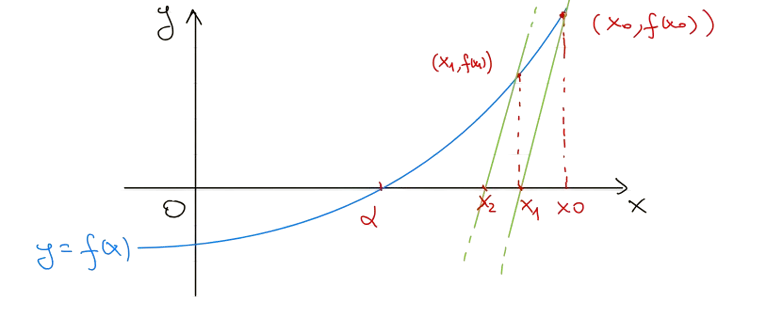
\includegraphics[width=1.0\textwidth]{images/direzione_costante}
\end{figure}
A partire da una stima iniziale $x_0$ di $\alpha$, si considera la retta passante per il punto $(x_0, f(x_0))$ è di coefficiente angolare $\frac{1}{m}$ con $m \neq 0$. La sua equazione sarà: 
\[
y - f(x_0) = \frac{1}{m}(x - x_0)
\]
Definiamo $x_1$ come l'intercetta di questa retta con l'asse delle ascisse:
\[
\begin{cases}
	y - f(x_0) = \frac{1}{m}(x - x_0) \\
	y = 0	
\end{cases}
\]
da cui \[x_1 = x_0 - mf(x_0)\]
Iterando la procedura si perviene al metodo della direzione costante:
\[
\begin{cases}
	x_0 \text{ assegnato } \\
	x_n = x_{n-1} - m(fx_{n-1})
\end{cases}
\]
La funzione iteratrice è:
\[
\phi(x) = x - mf(x)
\]
Essa dipende dal parametro $m$. Come deve essere scelto questo parametro per ottenere convergenza locale o globale? Risulta:
\[
\phi'(x) = 1 -mf'(x)
\]
\paragraph{Convergenza locale}
Dovremo imporre $|\phi'(\alpha)| < 1$.
\begin{align*}
	&-1 < 1 - mf'(\alpha) < 1 \\
	&-2 < -mf'(\alpha) < 0 \\
	&0 < mf'(\alpha) < 2
\end{align*}
Questa è la condizione per la convergenza locale.
\paragraph{Convergenza globale} Per la convergenza globale si ha il seguente risultato.
\begin{theorem}{\nmu Convergenza globale}{teorema_convergenza_globale}
	Sia $f \in C^1([a, b])$ tale che:
	\begin{enumerate}[label=(\alph*)]
		\item $f(a)f(b) < 0$
		\item $f'(x) \neq 0 \quad \forall x \in [a, b]$
		\item $0 < mf'(x) \leq 1 \quad \forall x \in [a,b]$
	\end{enumerate}
	Allora $f$ ammette un unico zero $\alpha \in (a,b)$ e il metodo della direzione costante converge globalmente ad $\alpha$ in tutto l'intervallo $[a, b]$. \\
\end{theorem}
\begin{proof}
	Dalla (c) ricaviamo:
\begin{align*}
	&0 < mf'(x) \leq 1 \\
	&-1 \leq -mf'(x) < 0 \\
	&0 \leq 1 - mf'(x) < 1 \\
	&0\leq \phi'(x) < 1
\end{align*}
Quindi la seconda ipotesi del teorema di convergenza globale è soddisfatta. Resta da provare $\phi([a, b]) \subset [a, b]$. \\
Poichè $\phi'(x) \geq 0$, $\phi(x)$ è monotona crescente e quindi
\[
a \leq x \leq b \Rightarrow \phi(a)  \leq \phi(x) \leq \phi(b)
\]
Si possono presentare i due casi nelle due figure sottostanti:
\begin{figure}[H]
	\centering
	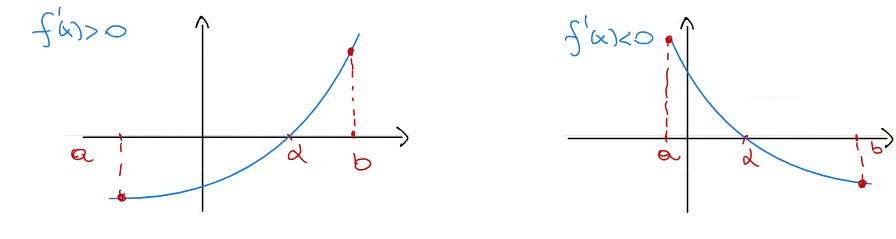
\includegraphics[width=1.0\textwidth]{images/casi_direzione_costante}
\end{figure}
Discutiamo il primo caso ($f'(x) > 0$). Risulta: 
\begin{align*}
	\phi(a) &= a - mf(a) > a \quad \text{in quanto $m > 0$ e $f(a) < 0$} \\
	\phi(b) &= b - mf(b) < b \quad \text{in quanto $m > 0$ e $f(b) > 0$} 
\end{align*}
In conclusione:
\[
a \leq x \leq b \Rightarrow a \leq \phi(x) \leq b
\]
\end{proof}
\section{Metodo di Newton (o delle tangenti)}
Definiamo questo metodo mediante due strategie diverse.
\subsection{Approccio analitico}
A partire da una stima iniziale $x_0$, sviluppiamo  $f(x)$ come polinomio di Taylor assestato al primo ordine in un intorno di $x_0$:
\[
f(x) = f(x_0) + f'(x_0)(x-x_0) + o(x - x_0)
\]
dove $o(x - x_0)$ denota un infinetisimo di ordine superiore al primo per $x \to x_0$:
\[
\lim\limits_{x \to x_0}\frac{o(x-x_0)}{x-x_0} = 0
\]
Se $x$ è vicino ad $x_0$, potremo trascurare l'infinitesimo $o(x-x_0)$ e scrivere 
\[
f(x) \approx f(x_0) + f'(x_0)(x-x_0)
\]
Anzichè risolvere $f(x) = 0$, risolveremo:
\[
f(x_0) + f'(x_0)(x-x_0) = 0
\]
Denotando con $x_1$ la soluzione, si ottiene:
\[
x_1 = x_0 - \frac{f(x_0)}{f'(x_0)}
\]
Iterando la procedura si ottiene il metodo di Newton:
\[
\begin{cases}
	x_0 \text{ assegnato}\\
	x_n = x_{n-1} - \frac{f(x_{n-1})}{f'(x_{n-1})}
\end{cases}
\]
Da cui, la funzione iteratrice è:
\[
\phi(x) = x - \frac{f(x)}{f'(x)}
\]
\subsection{Approccio geometrico}
\begin{figure}[H]
	\centering
	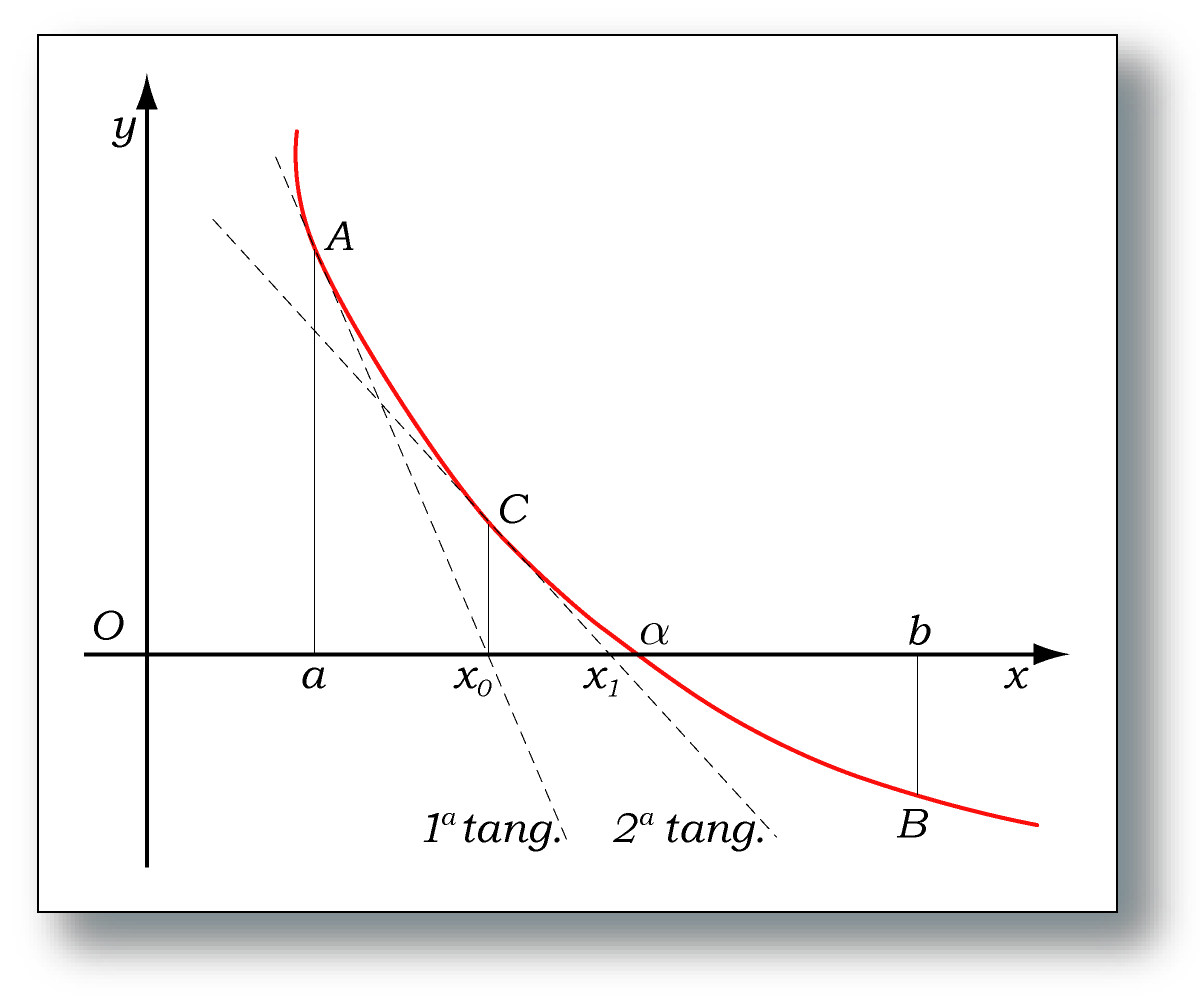
\includegraphics[width=0.8\textwidth]{images/metodo_newton}
\end{figure}
L'equazione della retta tangente al grafico di $f$ nel punto di ascissa $x_0$, è:
\[
y - f(x_0) = f'(x_0)(x - x_0)
\]
Denotiamo con $x_1$ l'intercetta della retta con l'asse $x$. Ponendo $y = 0$, si ottiene:
\[
x_1 = x_0 - \frac{f(x_0)}{f'(x_0)}
\]
Iterando la procedura si ottiene il metodo di Newton. \\
Studiamo la convergenza locale del metodo di Newton. Premettiamo la seguente definizione.
\begin{definition}{\nmu Molteplicità di uno zero}{molteplicita_zero}
	Sia $f \in C^d(B(\alpha, \delta))$ con $\alpha$ zero di $f$. \\
	La molteplicità (o ordine) dello zero di $\alpha$ di $f$ è un intero $d$ tale che:
	\[
	f(\alpha) = f'(\alpha) = \dots = f^{(d-1)}(\alpha) = 0 \wedge f^{(d)}(\alpha) \neq 0
	\]
\end{definition}
\paragraph{Significato analitico} Consideriamo lo sviluppo del polinomio di Taylor di $f$ in un intorno di $\alpha$:
\[
f(x) = f(\alpha) + f'(\alpha)(x-\alpha) + f''(\alpha)\frac{(x-\alpha)^2}{2!} + \dots + f^{(d-1)}(\alpha)\frac{(x-\alpha)^{d-1}}{(d-1)!} + f^{(d)}(\eta_x)\frac{(x-\alpha)^d}{d!}
\]
Poichè la molteplicità di $\alpha$ è $d$, risulta:
\[
f(x) = \frac{f^{(d)}(\eta_x)}{d!}(x-\alpha)^d
\]
con $\eta_x$ opportuno punto tra $x$ e $\alpha$. \\
Poichè $f^{(d)}(\alpha) \neq 0$, per $x \approx \alpha$ anche $f^{(d)}(\eta_x) \neq 0$. Osserviamo che in un intorno di $\alpha$, $f(x)$ si comporta come
\[
f(x) \approx cost. (x-\alpha)^d
\]
e quindi
\[
f(x) = 0 \sim (x -\alpha)^d = 0
\]
\paragraph{Interpretazione geometrica}
Se $d = 1$ allora $f(\alpha) = 0 \wedge f'(\alpha) \neq 0$ \\
\begin{figure}[H]
	\centering
	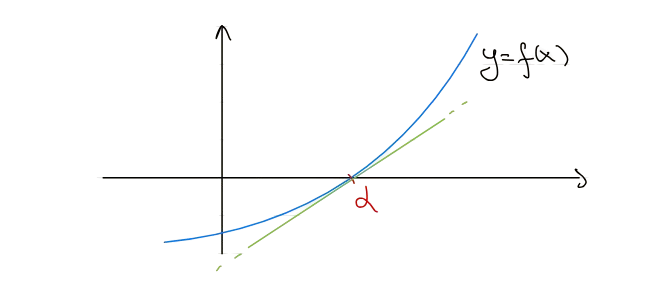
\includegraphics[width=1.0\textwidth]{images/zero_semplice}
\end{figure}
In tal caso $\alpha$ si dice zero semplice e questo è il caso più frequente. \\
Se $d = 2$ allora $f(\alpha) = f'(\alpha) = 0 \wedge f''(\alpha) \neq 0$ \\
\begin{figure}[H]
	\centering
	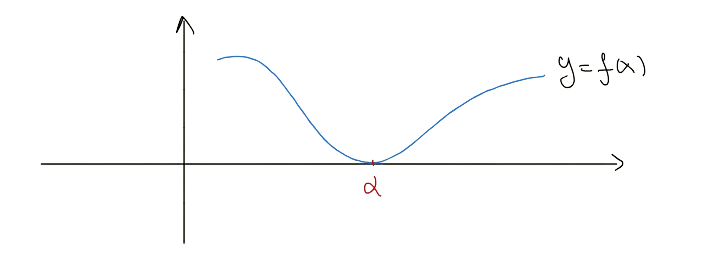
\includegraphics[width=1.0\textwidth]{images/zero_doppio}
\end{figure}
In questo caso $\alpha$ si dice zero doppio. \\
Se $d=3$ allora $f(\alpha) = f'(\alpha) = f''(\alpha) \wedge f'''(\alpha) \neq 0$ \\
\begin{figure}[H]
	\centering
	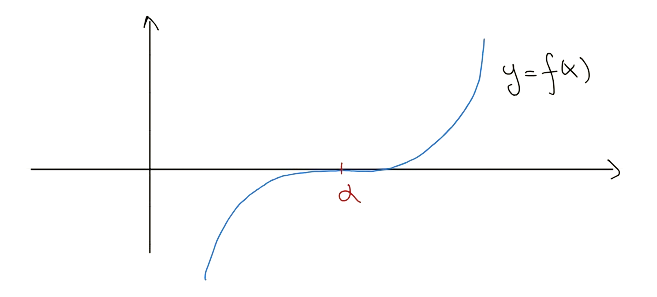
\includegraphics[width=1.0\textwidth]{images/zero_triplo}
\end{figure}
Torniamo al metodo di Newton. 
\[
\phi(x) = x - \frac{f(x)}{f'(x)}
\]
La sua derivata prima è:
\[
\phi'(x) = 1 - \frac{[f'(x)]^2 - f(x) \cdot f''(x)}{[f'(x)]^2} = \frac{f(x) \cdot f''(x)}{[f'(x)]^2}
\]
Distinguiamo due casi:
\begin{enumerate}
	\item $\alpha$ zero semplice: $f(\alpha) = 0 \wedge f'(\alpha) \neq 0$ \\
	Possiamo calcolare:
	\[
	\phi'(\alpha) = \frac{f(\alpha)\cdot f''(\alpha)}{[f'(\alpha)]^2} = 0
	\]
	Dal teorema di convergenza locale, concludiamo che il metodo di Newton è localmente convergente. 
	\item $\alpha$ zero di molteplicità $d \geq 2$:
	\[
	f(\alpha) = f'(\alpha) = \dots = f^{(d-1)}(\alpha) = 0 \wedge f^{(d)}(\alpha) \neq 0
	\]
	$\phi'(x)$ non è definita in $\alpha$ poichè il denominatore si annulla. Tuttavia, è possibile dimostrare che:
	\[
	\lim\limits_{x \to \alpha} \phi'(x) = 1 - \frac{1}{d}
	\]
	Possiamo prolungare la $\phi'(x)$ per continuità in $\alpha$, ponendo, per definizione:
	\[
	\phi'(\alpha) = \lim\limits_{x\to\alpha}\phi'(\alpha) = 1 - \frac{1}{d}
	\]
	Anche in questo caso risulta che $|\phi'(\alpha)| < 1$ e otteniamo la convergenza locale. 
\end{enumerate}
Quindi, concludendo, il metodo di Newton è sempre localmente convergente, pertanto, studiamone la convergenza globale. 
\begin{theorem}{\nmu Convergenza globale del metodo di Newton}{newton_conv_globale}
	Sia $f \in C^2([a, b])$ tale che:
	\begin{enumerate}[label=(\alph*)]
		\item $f(a)\cdot f(b) < 0$ 
		\item $f'(x) \neq 0 \quad \forall x \in [a, b]$
		\item $f''(x) \neq 0 \quad \forall x \in [a, b]$
	\end{enumerate}
	Allora $f$ ammette un unico zero $\alpha \in (a, b)$. Inoltre, scelto $x_0 \in [a, b]$ tale che $f(x_0) \cdot f''(x) > 0$, il metodo di Newton genera una successione $\{x_n\}$ che converge ad $\alpha$ monotonicamente.
\end{theorem}
\begin{proof} L'esistenza e l'unicità dello zero $\alpha \in (a, b)$ di $f$ discende dalle ipotesi (a) e (b). \\
	Si distinguono quattro casi schematizzati nei grafici sottostanti: \\
	\begin{figure}[H]
		\centering
		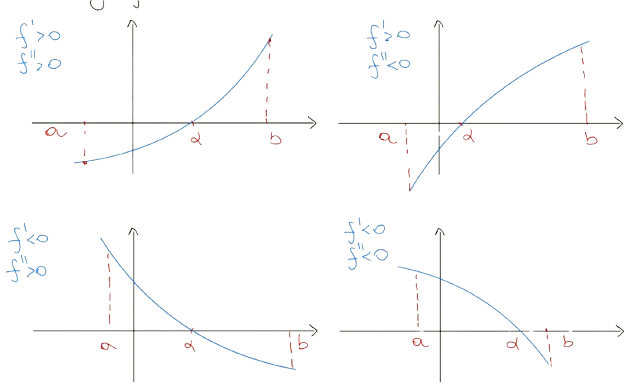
\includegraphics[width=1.0\textwidth]{images/newton_cong_globale}
	\end{figure}
	Esaminiamo il primo caso, $f'(x) > 0$ e $f''(x) > 0$. Ricordiamo che:
	\[
	\phi(x) = x - \frac{f(x)}{f'(x)} \quad \phi'(x) = \frac{f(x) \cdot f''(x)}{[f'(x)]^2}
	\]
	Dall'enunciato del teorema, dovremo scegliere $x_0 \in (\alpha, b]$. Facciamo innanzitutto vedere che $\phi((\alpha, b]) \subset (\alpha, b]$ \\
	Poichè in $(\alpha, b]$ risulta $\phi'(x) > 0$, ne consegue che $\phi$ è strettamente crescente in $(\alpha, b]$, quindi:
	\[
	\alpha < x \leq b \Rightarrow \phi(\alpha) < \phi(x) \leq \phi(b)
	\]
	Ora:
	\begin{align*}
		\phi(\alpha) &= \alpha \\
		\phi(b) &= b - \frac{f(b)}{f'(b)} < b \quad \text{in quanto} f(b) > 0\text{ e } f'(b) >0
	\end{align*}
	Abbiamo provato che $\alpha < \phi(x) < b$ \\
	Facciamo infine vedere che $\{x_n\}$ converge ad $\alpha$ ed è una successione strettamente decrescente. \\
	Dal punto precedente sappiamo che $x_n \in (\alpha, b] \quad \forall n \geq 0$.
	\[
	x_n = x_{n-1} - \frac{f(x_{n-1})}{f'(x_{n-1})} < x_{n-1}
	\] 
	$\{x_n\}$ è strattamente decrescente e limitata inferiormente da $\alpha$. Dall'analisi ammetterà limite finito:
	\[
	\exists \lim\limits_{n\to\infty}x_n = \beta \geq \alpha
	\]
	Poichè $\beta$ è punto fisso di $\phi$, necessariamente dovrà essere $\beta = \alpha$.
\end{proof}
\begin{corollary}{}{}
	Nelle stesse ipotesi (a), (b) e (c) del teorema di \namerefl{th:newton_conv_globale}, se $x_0 \in [a, b]$ e $x_1 = \phi(x_0) \in [a, b]$, allora la successione $\{x_n\}$ converge ad $\alpha$.
\end{corollary}
\begin{proof}
	Facendo riferimento sempre al primo caso, se scegliamo $x_0 \in [a, \alpha)$, essendo $\phi'(x) < 0$ in $[a, \alpha)$ segue che $\phi(x)$ è strettamente decrescente e quindi:
	\[
	x_0 < \alpha \Rightarrow x_1  = \phi(x_0) > \phi(\alpha) = \alpha
	\]
	e quindi, dall'ipotesi $x_1 \in [a, b]$ segue che $x_1 \in (\alpha, b]$ e da questo punto in poi vale il teorema precedente. 
\end{proof}
\section{Ordine di convergenza} 
L'ordine di convergenza è uno strumento che ci consente di stimare la velocità con cui una successione convergente tende al suo valore limite. Questo strumento ci consentirà di confrontare i metodi iterativi in base alla rapidità di convergenza delle successioni che essi generano. 
\begin{definition}{\nmu Ordine di convergenza}{ordine_convergenza}
	Sia $\{x_n\}$ una successione convergente ad $\alpha \in \mathbbm{R}$:
	\[
	\lim\limits_{n\to\infty}x_n = \alpha \in \mathbbm{R}
	\]
	Si definisce \textit{ordine di convergenza} della successione $\{x_n\}$ un reale positivo $p > 0$ tale che esista e sia finito il seguente limite:
	\[
	\lim\limits_{n\to\infty}\frac{|x_{n+1} - \alpha|}{|x_n - \alpha|^p} = c
	\]
	con $0 < c < +\infty$
\end{definition}
Analizziamone il significato. Per $n$ abbastanza grande possiamo scrivere:
\[
\frac{|x_{n+1} - \alpha|}{|x_n - \alpha|^p} \approx c
\]
da cui:
\[
|x_{n+1}-\alpha| \approx c \cdot  |x_n - \alpha|^p
\]
Tale uguaglianza relaziona l'errore assoluto a un generico passo con l'errore assoluto al passo precedente e quindi esprime la legge con cui l'errore si riduce, per $n$ grande, ad ogni passo. Ne consegue che la riduzione dell'errore ad ogni passo sarà tanto maggiore:
\begin{itemize}
	\item quanto più grande è il valore di $p$;
	\item quanto più piccolo è il valore di $c$.
\end{itemize}
La costante $c$ è detta \textit{costante asintotica di convergenza}. La convergenza si dice:
\begin{itemize}
	\item lineare se $p = 1$;
	\item superlineare se $p > 1$;
	\item quadratica se $p = 2$
\end{itemize}
\begin{note}{}{}
	Se $p = 1$, necessariamente $0 < c < 1$. Infatti per $n$ grande, abbiamo:
	\[
	|x_{n+1}-\alpha| \simeq c|x_n-\alpha|
	\]
	Se $c >=1$, la distanza tra $x_n$ e $\alpha$ non si ridurrebbe al crescere di $n$, e ciò contraddice l'ipotesi che $x_n \to \alpha$
\end{note}
\begin{definition}{\nmu Ordine di convergenza di un metodo iterativo}{ordine_conv_iterativo}
	Un metodo iterativo per la ricerca degli zeri di una funzione si dice di ordine $p$ se, applicato a una data classe di funzioni, genera successioni che convergono allo zero con ordine $p$.
\end{definition}
\begin{example}{}{}
	Consideriamo due metodi iterativi one-step definiti dalle due iteratrici $\phi_1$ e $\phi_2$, e supponiamo che, applicati per la ricerca di uno zero $\alpha$ di una funzione $f$:
	\[
	\phi_1: p_1 =1 \text{ (convergenza lineare) e } c_1 = \frac{1}{10}
	\]
	\[
	\phi_2: p_2 =2 \text{ (convergenza quaratica) e } c_2 = 10
	\]
	Stiamo avvantaggiando il primo metodo relativo al valore della costante asintotica in quanto:
	\[
	c_2 = 100c_1
	\]
	Ipotesi di lvaoro: scegliamo, per i due metodi, una condizione iniziale $x_0$ tale che:
	\[
	|x_0 - \alpha| = 10^{-2}
	\]
	e supponiamo di trovarci in un intorno abbastanza piccolo di $\alpha$, in modo tale che
	\[
	|x_{n+1} -\alpha| \approx c|x_n - \alpha|^p
	\]
	Generiamo le due successioni.
	\begin{center}
		\begin{tabular}{c|c|c}
			$n$ & \textbf{Errore Assoluto} $\phi_1(x_n)$ & \textbf{Errore Assoluto} $\phi_2(x_n)$ \\ \hline
			0 & $10^{-2}$ & $10^{-2}$ \\
			1 & $\approx 10^{-3}$ & $\approx 10^{-3}$ \\
			2 & $\approx 10^{-4}$ & $\approx 10^{-5}$ \\
			3 & $\approx 10^{-5}$ & $\approx 10^{-9}$ \\
			4 & $\approx 10^{-6}$ & $\approx 10^{-17}$ \\
		\end{tabular}
	\end{center}
\end{example}
\begin{note}{}{}
	In caso di convergenza quadratica, se la costante asintotica $c \approx 1$, il numero di cifre significative dell'approssimazione allo zero $\alpha$, definitivamente raddoppia da un passo al successivo
	\[
	|x_{n+1}-\alpha|\approx c |x_n - \alpha|^2 \quad \text{ con } c \approx 1
	\]
	Se $\frac{|x_n-\alpha|}{|\alpha|} < 10^{-d}$, quindi $x_n$ contiene $d$ cifre significative corrette, abbiamo:
	\[
	\frac{|x_n-\alpha|}{|\alpha|} \approx \frac{|x_n - \alpha|^2}{|\alpha|} = |\alpha|\cdot\Bigg(\frac{|x_n-\alpha|}{|\alpha|}\Bigg)^2 < |\alpha|10^{-2d}
	\]
\end{note}
La seguente proposizione ci fornisce un modo per  determinare l'ordine di convergenza $p$ di un metodo iterativo nel caso di metodi iterativi one-step. 
\begin{proposition}{}{}
	Sia $\phi \in C^p(B(\alpha, \delta))$, con $\alpha$ punto fisso di $\phi$, Sono equivalenti le seguenti due proposizioni
	\begin{enumerate}[label=(\alph*)]
		\item Il metodo iterativo one-step definito da $\phi$ ha ordine $p$.
		\item $\phi'(\alpha)=\phi''(\alpha) = \dots = \phi^{(p-1)}(\alpha) = 0 \wedge \phi^{(p)}(\alpha) \neq 0$
	\end{enumerate}
\end{proposition}
\begin{proof}
	Delle due implicazioni $(a) \Rightarrow (b)$ e $(b) \Rightarrow (a)$, mostreremo solo al seconda, che è la più importante. \\
	$(b) \Rightarrow (a) \quad$ Consideriamo lo sviluppo di Taylor della funzione iteratrice $\phi$ in un intorno di $\alpha$:
	\[
	\phi(x) = \phi(\alpha) + \phi'(\alpha) + \frac{\phi''(\alpha)}{2!}(x-\alpha)^2 + \dots + \frac{\phi^{(p-1)}}{(p-1)!}(x-\alpha)^{p-1} + \frac{\phi^{(p)}(\eta_x)}{p!}(x-\alpha)^p
	\]
	Con $\eta_x$ opportuno punto tra $x$ e $\alpha$. \\
	Dall'ipotesi $(b)$ possiamo semplificare come:
	\[
	\phi(x) = \phi(\alpha) + \frac{\phi^{(p)}(\eta_x)}{p!}(x-\alpha)^p
	\]
	Per la successione $\{x_n\}$ generata dal metodo possiamo scrivere:
	\[
	x_{n+1} - \alpha = \phi(x_n) - \phi(\alpha) = \frac{\phi^{(p)}(\eta_n)}{p!}(x_n - \alpha)^p
	\]
	dove $\eta_n$ è un opportuno punto tra $x_n$ e $\alpha$. \\
	Si noti che, poichè $x_n \to \alpha$, anche $\eta_n \to \alpha$. Otteniamo che:
	\begin{align*}
		\lim\limits_{n\to\infty}\frac{|x_{n+1} - \alpha|}{|x_n - \alpha|^p} &= \lim\limits_{n\to\infty}\frac{|\phi^{(p)}(\eta_n)|}{p!} \\
		&= \frac{1}{p!}|\phi^{(p)}(\lim\limits_{n\to\infty}\eta_n)| \\
		&= \frac{1}{p!}|\phi^{(p)}(\alpha)|
	\end{align*}
\end{proof}
\begin{note}{}{}
	La costante asintotica di convergenza dei metodi one-step è:
	\[
	\frac{1}{p!}|\phi^{(p)}(\alpha)|
	\]
	In particolare, per $p =1$,
	\[
	c = |\phi'(\alpha)|
	\]
\end{note}
\subsection{Metodo della direzione costante}
Ricordiamo che:
\begin{align*}
	\phi(x) &= x - mf(x) \\
	\phi'(x) &= 1 - mf'(x) \\
	\phi'(\alpha) = 1 - mf'(\alpha)
\end{align*}
Distinguiamo due casi:
\begin{enumerate}
	\item $m \neq \frac{1}{f'(\alpha)}$. Questo è il caso generale. Risulta $\phi'(\alpha) \neq 0$ e quindi l'ordine di convergenza è $p = 1$. 
	\item $ m = \frac{1}{f'(\alpha)}$.  In questo caso eccezionale risulta $\phi'(\alpha) = 0$ e quindi la successione $\{x_n\}$ generata con questa scelta converge ad $\alpha$ con ordine $p = 2$. 
\end{enumerate}
L'ordine di convergenza del metodo della direzione costante è $p = 1$.
\subsection{Metodo di Newton}
Ricordiamo che:
\begin{align*}
\phi(x) &= x - \frac{f(x)}{f'(x)} \\
\phi'(x) &= \frac{f(x) \cdot f''(x)}{[f'(x)]^2}
\end{align*}
Distinguiamo due casi:
\begin{enumerate}
	\item $\alpha$ zero semplice. In questo caso generale:
	\[
	\phi'(\alpha) = 0
	\]
	In generale, $\phi'(\alpha) = 0$, quindi il metodo di Newton, in presenza di zeri semplici, ha ordine $p = 2$.
	\item $\alpha$ zero di molteplicità $d > 1$. In tal caso, avevamo provato che:
	\[
	\phi'(\alpha) = \lim\limits_{x\to\alpha}\phi'(x) = 1 - \frac{1}{d} \neq 0
	\] 
	In presenza di zeri multipli, la successione $\{x_n\}$ generata dal metodo di Newton converge ad $\alpha$ linearmente. 
\end{enumerate}
Quindi il vantaggio del metodo di Newton è che esso converge con ordine $p = 2$. Tuttavia, per la sua implementazione, occorre preventivamente calcolare la derivata prima di $f$. Ciò può essere oneroso se $f$ ha un'espressione complicata o addirittura impossibile se $f$ non è nota. Inoltre, il costo computazionale per iterata del metodo di Newton è:
\[
\frac{2\text{ valutazioni di funzione}}{\text{iterata}}
\]
quindi, ad esempio, costa il doppio rispetto al metodo della direzione costante. Si osservi che il numero di valutazioni di funzione è proporzionale al tempo di esecuzione sul calcolatore. Infine, la convergenza del metodo può rallentare molto se $x_n$ non è abbastanza vicino ad $\alpha$. In alcuni casi la regione di convergenza potrebbe essere molto piccola, il chè richiederebbe una stima iniziale $x_0$ molto buona.  \\
Per questo, si introducono alcune varianti del metodo di Newton che possono risolvere uno o più degli svantaggi sopra elencati. Ne analizziamo due.
\section{Metodo di Newton modificato}
Il metodo di Newton modificato non è altro che il metodo della direzione costante con la seguente definizione del parametro $m$:
\[
m = \frac{1}{f'(x_0)}
\]
Il metodo di Newton modificato è:
\[
\begin{cases}
	x_0 \text{ assegnato} \\
	x_n = x_{n-1} - \frac{f(x_n)}{f'(x_0)} & n \geq 1
\end{cases}
\]
La derivata prima di $f$ va calcolata solo nel punto iniziale. L'idea è che se $x_0 \approx \alpha$ allora $f'(x_0) \approx f'(\alpha)$ e quindi
\[
m = \frac{1}{f'(x_0)} \approx \frac{1}{f'(\alpha)}
\] 
Ricordiamo che per $m = \frac{1}{f'(\alpha)}$ la convergenza sarebbe quadratica. Nel nostro caso, il metodo diventa lineare, ma la costante asintotica è piccola:
\[
|\phi'(\alpha)| = |1 - mf'(\alpha)| = \Bigg|1 - \frac{f'(\alpha)}{f'(x_0)}\Bigg| \ll 1
\]
Il costo computazionale è pari a:
\[
\frac{\text{1 valutazione di funzione}}{\text{iterata}}
\]
\section{Metodo delle secanti}
Il metodo delle secanti lo si ottiene dal metodo di Newton operando la seguente approssimazione della derivata prima di $f$ in $x_n$:
\[
f'(x_n) \approx \frac{f(x_n) - f(x_{n-1})}{x_n - x_{n-1}}
\]
Il metodo delle secanti è così definito:
\[
\begin{cases}
	x_0, x_1 \text{ assegnati}, \\
	x_{n+1} = x_n - \frac{f(x_n)}{\frac{f(x_n) - f(x_{n-1})}{x_n - x_{n-1}}}, & n \geq 1
\end{cases}
\]
È un metodo a due passi. Si può dimostrare che il suo ordine è:
\[
p = \frac{1 + \sqrt{5}}{2}
\]
Si tratta di un metodo superlineare $1 < p < 2$. Il costo computazionale è:
\[
\frac{\text{1 valutazione di funzione}}{\text{iterata}}
\]
Vediamo il perchè di questo risultato.
\paragraph{Interpretazione geometrica} 
\begin{figure}[H]
	\centering
	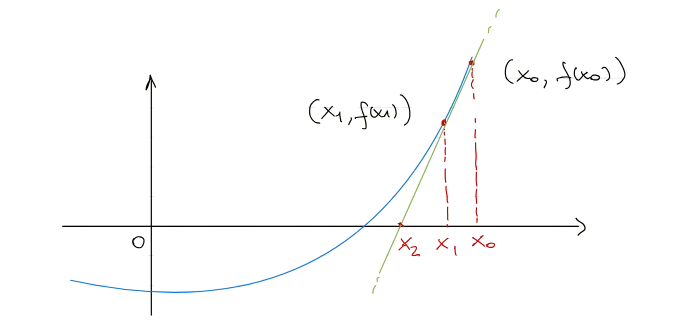
\includegraphics[width=1.0\textwidth]{images/secanti_geometrico}
\end{figure}
Il punto $x_2$ lo si ottiene come intercetta della retta secante il grafico della funzione $f$ nei punti di ascissa $x_0$ e $x_1$. L'equazione di questa retta è:
\[
y - f(x_0) = \frac{f(x_1) - f(x_0)}{x_1 - x_0}(x - x_0)
\]
\paragraph{Criteri di arresto}
Poichè non possiamo calcolare gli infiniti elementi della successione $\{x_n\}$ ed inoltre, considerando che il calcolatore ha una precisione finita, arresteremo l'iterazione quando
\[
|x_n - \alpha| < tol
\]
dove tol è una tolleranza assegnata in input dall'utente. Un'analoga condizione possiamo scriverla per l'errore relativo e per l'errore misto. Per il momento consideriamo l'errore assoluto. Quando la condizione sopra scritta si realizza, il processo di iterazione ha termine e si considera l'ultimo elemento calcolato della successione quale approssimante di $\alpha$:
\[
x_n \approx \alpha
\]
Poichè $\alpha$ non è noto, la condizione di arresto non è una condizione operativa. Si possono seguire due strade:
\begin{enumerate}
	\item determinare una maggiorazione calcolabile dell'errore assoluto;
	\item determinare una stima dell'errore assoluto. 
\end{enumerate}
\paragraph{Maggiorazione dell'errore assoluto} Consideriamo
\begin{align*}
x_{n+1} - x_n &= x_{n+1} - \alpha + \alpha - x_n \\
&= \phi(x_n) - \phi(\alpha) - (x_n - \alpha) \\
&= \phi'(\eta_n)(x_n - \alpha) - (x_n - \alpha) \\
&= (\phi'(\eta_n) - 1)(x_n - \alpha)
\end{align*}
Poichè $\eta_n \to \alpha$ per $n \to \infty$ ciò implica che $|\phi'(\eta_n)| < 1$ per $n$ grande e quindi, per $n$ grande
\[
1 - \phi'(\eta_n) \geq 1 - |\phi'(\eta_n)| > 0
\]
Dalle uguaglianze precedenti ricaviamo:
\[
|x_n - \alpha| = \frac{1}{|1-\phi'(\eta_n)|}|x_{n+1} - x_n| \leq \frac{1}{1-|\phi'(\eta_n)|}|x_{n+1} - x_n|
\]
Se si riesce a determinare un intervallo $[a, b]$ tale che:
\begin{itemize}
	\item $\alpha \in (a, b)$ 
	\item $|\phi'(x)| < 1$ in $[a, b]$
\end{itemize}
Denotando con $M = \max_{a \leq x \leq b}|\phi'(x)| < 1$ per $n$ grande $\eta_n \in (a, b)$ e quindi:
\begin{align*}
	|\phi'(\eta_n)| &\leq M \\
	-|\phi'(\eta_n)| &\geq M \\
	1 - |\phi'(\eta_n)| &\geq 1 - M \\
	\frac{1}{1- |\phi'(\eta_n)|} &\leq \frac{1}{1- M}
\end{align*}
Sfruttando questa maggiorazione otteniamo
\[
|x_n - \alpha| \leq \frac{1}{1-M} |x_{n+1}-x_n|
\]
Abbiamo ottenuto due maggioranze valutabili dell'errore assoluto. Il criterio di arresto diventa
\[
\frac{1}{1-M}|x_{n+1} - x_n| < tol
\]
\paragraph{Stima dell'errore} Anzichè determinare una maggiorazione dell'errore, se ne determina una stima. In generale si sceglie:
\[
|x_n - \alpha| \approx C|x_{n+1}-x_n|
\]
$C$ è una costante solitamente fissata ad $1$ oppure $C > 1$. La scelta $C = 1$ è certamente appropriata per il metodo di Newton. Infatti sappiamo che, in presenza di zeri semplici, $\phi'(\alpha) = 0$; ciò significa che, per $n$ grande, $\phi'(\eta_n) \approx 0$ e quindi
\[
\frac{1}{1 - \phi'(\eta_n)} \approx 1
\] 
Scegliendo $C = 1$, il criterio di arresto si semplifica come:
\[
|x_{n+1}-x_n|  < tol
\] 
Per l'errore relativo, possiamo usare il seguente criterio di arresto:
\[
\frac{|x_{n+1}-x_n|}{|x_{n+1}|} < tol
\]
Infine, per l'errore misto:
\[
\frac{|x_{n+1}-x_n|}{1 + |x_{n+1}|} < tol
\]
\chapter{Richiami sui numeri complessi}
\chapter{Aritmetica di macchina e analisi degli errori}
\section{Considerazioni preliminari}
Per la rappresentazione dei numeri reali si utilizza, solitamente, una notazione posizionale. Ad esempio:
\[
123.45 = 1\cdot 10^2 + 2 \cdot 10 + 3 \cdot 10^0 + 4 \cdot 10^{-1} + 5 \cdot 10^{-2}
\]
Più in generale, lavorando con una base $\beta \geq 2$:
\[
d_md_{m-1} - d_0.d_1d_2\dots d_n = d_n\beta^m + d_{m-1}\beta^{m-1} + \dots + d_0\beta^0 + d_1\beta^{-1} + \dots + d_n\beta^{-n}
\]
Consideriamo il seguente esempio.
\begin{example}{}{}
	Supponiamo che, per la memorizzazione dei numeri reali abbiamo a dispozione un campo di memoria costituito da 5 celle, ciacsuna delle quali può ospitare una cifra. Consideriamo il seguente esempio:
	\[
	x = 0.00123456
	\]
	Nel campo di memoria assegnato, il numero $x$ verrà rappresentato dalla sua approssimazione
	\[
	x_1 = 0.0012 \simeq x
	\]
	Considerando invece la rappresentazione normalizzata di $x$:
	\[
	x = 1.23456 \cdot 10^{-3}
	\]
	Utilizzando questa notazione, potremo dedicare una cella per la memorizzazione dell'esponente, ottendo così l'approssimazione
	\[
	x_2 = 1.234 \cdot 10^{-3}
	\]
	È evidente che $x_2$ risulta una migliore approssimazione di $x$ rispetto a $x_1$. Quindi, per la rappresentazione dei numeri reali converrà utilizzare la notazione normalizzata:
	\[
	x = \pm d_0.d1d_2\cdots\beta^p
	\]
	ove $d_0.d1_d2\cdots$ è la \textit{mantissa}, $\beta$ è la \textit{base} e $p$ è l'\textit{esponente}, il cui significato è:
	\[
	x = \pm \beta^p\sum_{i=0}^{\infty}d_i\beta^{-i}
	\]
	con $d_0 \neq 0$
\end{example}
\begin{theorem}{\nmu Rappresentazione in base}{rappr_base}
	Sia $\beta \geq 2$ ove $\beta$ è un intero. Allora, ogni numero reale $x \in \mathbbm{R}$, $x \neq 0$ può esesre espresso in maniera univoca come
	\[
	x = \pm\beta^p \sum_{i=0}^{\infty}d_i\beta^{-i}
	\]
	dove:
	\begin{itemize}
		\item $\beta$ è la \textit{base della rappresentazione};
		\item $p \in \mathbbm{Z}$ è l'\textit{esponente};
		\item $\pm$ è il \textit{segno};
		\item $0 \leq d_i \leq \beta - 1$, $i = 0,1, \dots$
		\item $d_0 \neq 0$ detta \textit{condizione di normalizzazione};
		\item le cifre $d_i$ non sono definitivamente uguali a $\beta - 1$.
	\end{itemize}
\end{theorem}
\begin{note}{}{}
	\begin{enumerate}
		\item Abbiamo escluso lo zero poichè questo non ammette una notazione normalizzata.
		\item L'ultima condizione impone che le cifre $d_i$ non siano uguali a $\beta - 1$ da un certo indice in poi. Tale condizione è importante per avere l'unicità della rappresentazione.  
	\end{enumerate}
\end{note}
\begin{example}{}{}
	In base $\beta = 10$, scegliamo il numero 
	\begin{align*}
		x &= 0.\overline{9} = 9.\overline{9} \cdot 10^{-1} \\
		&= 10^{-1} \sum_{i=0}^{\infty}9 \cdot 10^{-i} = \frac{9}{10}\sum_{i=0}^{\infty}\Bigg(\frac{1}{10}\Bigg)^i \\
		&= \frac{9}{10}\frac{1}{1-\frac{1}{10}} = 1
	\end{align*}
	In conclusione $0.\overline{9}$ e 1 rappresentano lo stesso  numero reale. Analogamente:
	\[
	1.23\overline{9} = 1.24
	\]
	Il calcolatore, disponendo di memoria finita, non può rappresentare correttamente gli infiniti numeri reali. Le difficoltà nascono da due impedimenti:
	\begin{itemize}
		\item il numero arbitriaramente elevato delle cifre $d_i$
		\item l'esponente $p$ può variare da $-\infty$ a $+\infty$
	\end{itemize}
	Dovremo quindi fissare un numero massimo di cifre $d_i$ e una variabilità finita per l'esponente.
\end{example}
\section{Numeri di macchina}
Sono quei numeri reali che il calcolatore è in grado di rappresentare correttamente. 
\begin{definition}{\nmu Insieme dei numeri di macchina}{insieme_numeri_macchina}
	Siano $\beta \geq 2$, $t \geq 0$, $M_1, M_2$ interi. \\
	Si definisce insieme dei numeri di macchina in base $\beta$, con $t + 1$ cifre significative e range per l'esponente $p \in (M_1, M_2)$, il seguente sottoinsieme di $\mathbbm{R}$:
	\[
	\mathbbm{F} = \{ x \in \mathbbm{R} \mid x = \pm \beta^p\sum_{i=0}^{t}d_i\beta^{-i}\} \cup \{0\}
	\] 
	dove:
	\begin{itemize}
		\item $\beta$ è la base della rappresentazione;
		\item $\pm$ è il segno;
		\item $ 0 \leq d_i \leq \beta -1$, $d_0 \neq 0$
		\item $p \in  (M_1, M_2)$
	\end{itemize}
\end{definition}
Osserviamone alcune proprietà.
	\begin{enumerate}
		\item $card(\mathbbm{F}) < +\infty$, $\mathbbm{F}$ è un sottoinsieme finito di $\mathbbm{R}$.
		\item Al fine di memorizzare numeri piccoli (con esponente negativo) e grandi (con esponente positivo), sceglieremo $M_1 < 0$ e $M_2 > 0$
		\item Per la base $\beta$, i calcolatori utilizzano generalmente il sistema binario. \\
		Questa scelta è suggerita dalla natura fisica dei dispositivi elettronici che memorizzano ed elaborano i dati. Essi possono assumere due stati fisici. Ad esempio:
		\begin{itemize}
			\item passaggio o meno di corrente attraverso una resistenza;
			\item magnetizzazione o meno di un dispositivo magnetico.
		\end{itemize}
		\item Un vantaggio dell'uso del sistema binario è che, dovendo essere $d_i = 0, 1$, dalla condizione di normalizzazione:
		\[
		d_0 \neq 0 \Rightarrow d_0 = 1
		\]
		quindi è inutile memorizzare la cifra $d_0$ risparmiando così 1 bit.
		\item I numeri di macchina sono disposti simmetricamente rispetto alla zero, tuttavia la loro distribuzione non è uniforme. Più in particolare consideriamo un generico numero di macchina positivo:
		\[
		a = \beta^p\sum_{i=0}^{t}d_i\beta^{-i}
		\]
		Il numero di macchina successivo, lo denotiamo con \textit{b}, lo si ottiene incremente di una unità l'ultima cifra $d_t$:
		\begin{align*}
			b &= a + \beta^p \cdot 0.0\dots1 \\
			&= a + \beta^p\beta^{-t} = a + \beta^{p-t}
		\end{align*}
		da cui, la distanza tra due numeri di macchian consecutivi è
		\[
		b - a = \beta^{p-t}
		\]
		Notiamo che questa distanza dipende dalla grandezza del numero di macchina consdirato per la presenza dell'esponente $p$. Ne consegue che i numeri di macchina sono più densi vicino all'origine e si diradano man mano che ci allontaniamo dall'origine.
		\item Utilizzando la notazione posizionale un numero di macchina non nulla ha l'espressione:
		\[
		x = \pm\beta^p(d_0.d1\dots d_t)
		\]
		Determiniamo il $\min{\mathbbm{F}_+^*}, \max{\mathbbm{F}_+^*}$ dove $\mathbbm{F}_+^*$ denota l'insieme dei numeri di macchina positivi. \\
		Siano $\omega = \min{\mathbbm{F}_+^*}, \Omega = \max{\mathbbm{F}_+^*}$. \\
		$\omega$ lo si ottiene minimizzando i valori dell'esponente $p$ e della mantissa. Pertanto:
		\[
		\omega = \beta^{M_1 + 1}1.0\dots0 = \beta^{M_1 + 1}
		\]
		Per determinare $\Omega$ premettiamo la seguente proprietà. Sia $z \neq 1$; risulta:
		\begin{align*}
		1 + z + \dots + z^t &= \frac{(1-z)(1+z+\dots+z^t)}{1-z} \\
		&= \frac{1 + z + z^2 + \dots + z^t  - z -z^2 - \dots - z^{t + 1}}{1-z} \\
		&= \frac{1 - z^{t+1}}{1-z}
		\end{align*}
		Questa è la formula di una progressione geometrica di ragione $z$. Passiamo al calcolo di $\Omega$:
		\begin{align*}
			\Omega &= \beta^{M_2 - 1}\sum_{i=0}^{t}(\beta -1)\beta^{-i} = \beta^{M_2 - 1}(\beta - 1)\sum_{i=0}^{t}(\beta^{-1})^i \\
			&= \beta^{M_2 - 1}(\beta - 1)\frac{1 - \beta^{-t - 1}}{1 - \beta^{-1}} \\
			&= \beta^{M_2}(1 - \beta^{-t - 1}) \text{ oppure } \beta^{M_2 - 1}(\beta - \beta^{-t})
		\end{align*}
	\end{enumerate}
\section{Standard IEEE-754}
Lo standard IEEE-754 è uno standard per l'implementazione dell'aritmetica di macchina sui calcolatori, al fine di rendere compativili i codici sulle varie piattaforme. Questo standard prevede le seguenti due modalità fondamentali:
\begin{itemize}
	\item Semplice (o singola) precisione;
	\item Doppia precisione.
\end{itemize}
La doppia precisione è la modalità più frequentemente utilizzata. In ogni caso la base utilizzata è $\beta = 2$.
\subsection{Semplice precisione}
In semplice precisione, per la memorizzazione di un numero di macchina, viene predisposto un campo di memoria costituito da 32 bit così suddivisi:
\begin{itemize}
	\item 1 bit per il segno;
	\item 8 bit per l'esponente;
	\item 23 bit per la mantissa.
\end{itemize}
Il segno viene rappresentato mediante 0 per il più e 1 per il meno. \\
Con un'esponente di 8 bit possiamo realizzare $2^8 = 256$ configurazioni distinte. Si sceglie:
\[
M_1 = -127 \quad M_2 = 128
\]
Anzichè memorizzare l'esponente con il suo segno, si applica una tecnica di traslazione (bias) in base alla quale viene memorizzata la cosiddetta \textit{caratteristica} $p^*$ che è relazionata all'esponente $p$ mediante l'equazione
\[
p^* = p - M_1 \iff p = p^* + M_1
\]
La seguente tabella chiarisce meglio i termini di questa relazione. \\
\textbf{Fare tabella} \\
La configurazione vuota $(p^* = 0)$ e quella piena $(p^* = 255)$ sono state lasciate libere. Esse sono utilizzate per altri scopi:
\begin{itemize}
	\item lo zero si rappresenta con caratteristica nulla e mantissa nulla.
	\item la caratteristica piena serve per gestire le cosidette eccezioni previste dallo standard IEEE:
	\begin{itemize}
		\item $p^* = 255$ e mantissa nulla identificano il simbolo $+Inf$
		\item $P^* = 255$ e mantissa non nulla identificano il simbolo $NaN$ 
	\end{itemize}
	Questi simboli sono l'output di alcune operazioni non consentite in aritmetica reale e il loro scopo è evitare l'arresto dell'esecuzione di un codice in corrispondenza di queste operazioni. Ad esempio:
	\[
	\frac{1}{0} = +Inf \quad \tan\frac{\pi}{2} = +Inf
	\]
	\[
	\arctan(+Inf) = \frac{\pi}{2}
	\]
	\[
	\frac{0}{0} = NaN; \quad Inf - Inf = NaN
	\]
	\[
	1^{Inf} = Nan \quad \frac{Inf}{Inf} = Nan
	\]
	\item Scegliendo caratteristica nulla e mantissa non nulla, si identificano i cosidetti \textbf{numeri subnormali} o  non normalizzati. I numeri subnormali sono numeri non normalizzati, quindi con $d_0 = 0$ più piccoli ma molto prossimi a $\omega$. \\
	Sono utilizzati per memorizzare numeri  reali più piccoli ma molto prossimi ad $\omega$ meglio di quanto non facciano lo zero e lo stesso $\omega$. \\
	L'espressione generica di un numero subnormale è:
	\[
	\pm \beta^{M_1 + 1}0.d_1d_2\dots d_t
	\]
	Ad esempio, il più grande numero subnormale lo si ottiene scegliendo $d_1 = d_2 = \dots = d_t = \beta - 1$ \\
	Il più piccolo numero subnormale positivo è: $\beta^{M_1 + 1 - t}$
\end{itemize}
\subsection{Doppia precisione}
A ogni numero di macchina viene riservato un campo costituito da 64 bit così suddivisi:
\begin{itemize}
	\item 1 bit per il segno;
	\item 11 bit per l'esponente;
	\item 52 bit per la mantissa.
\end{itemize}
Per l'esponente $p$ si sceglie il seguente range:
\[
M_1 = -1023 \quad M_2 = 1024
\]
Ne consegue che, in doppia precisione:
\[
\omega = 2^{-1022} \approx 2.2 \cdot 10^{-308}
\]
\[
\Omega = 2^{1024}(1 - 2^{-53}) \approx 1.7\cdot 10^{308}
\]
In doppia precisione, i numeri subnormali sono:
\[
\omega = 2^{-1022}\cdot 1.0\dots0
\]
\begin{align*}
\text{subnormali } & 2^{-1022} \cdot 0.1\dots 1 \\
& \vdots \\
& 2^{-1022}\cdot 0.0\dots01 \\
&= 2^{-1074}
\end{align*}
\begin{note}{}{}
	I numeri subnormali hanno un numero di cifre significative minore di $t + 1$. In effetti la presenza degli zeri all'inizio della mantissa serve per perfezionare l'esponente permettendogli di assumere valori minori di $M_1 + 1$ a discapito di una perdita di accuratezza in termini di cifre significative. 
\end{note}
\section{Rappresentazione dei numeri reali mediante i numeri di macchina}
Ogni numero reale verrà approssimato sul calcolatore mediante un opportuno numero di macchina. Occorre definire una funzione;
\[
fl: \mathbbm{R} \to \mathbbm{F}
\]
Distinguiamo i seguenti casi. Sia $x \in \mathbbm{R}$ e, senza ledere la generalità, supponiamo $x > 0$, sfruttando la simmetria di $\mathbbm{F}$. Possiamo scrivere:
\[
x = \beta^p\sum_{i=0}^{\infty}d_i\beta^{-i}
\]
\begin{enumerate}
	\item $x\in\mathbbm{F}$. In tal caso, ovviamente, porremo $fl(x) = x$ \\
	In altri termini,
	\[
	fl|_\mathbbm{F} = \text{identità}
	\]
	\item $p \geq M_2$. L'esponente di $x$ è più grande del numero esponente consentito in $\mathbbm{F}(M_2 - 1)$. Si genera una condizione di \textit{overflow} e si pone
	\[
	fl(x) = +Inf
	\]
	\item $p \leq M_1$. L'esponente di $x$ è più piccolo del minimo esponente consentito in $\mathbbm{F}(M_1 + 1)$. Si genera una condizione di \textit{underflow} e si pone
	\[
	fl(x) = \begin{cases}
		\text{subnormale} & M_1 - t + 1 \leq p \leq M_1 \\
		0 & p \leq M_1 - t
	\end{cases}
	\]
	Ora analizziamo il caso più frequente.
	\item $M_1 < p < M_2, x\in\mathbbm{F}$. Ciò significa che $\exists i > t$ tale che $d_i \neq 0$ \\
	Si possono presentare due sottocasi
	\begin{enumerate}
		\item $x\in(\omega, \Omega)$
		\item $p = M_2 - 1$, $d_0 = d_1 = \dots = d_t = \beta - 1$ e $\exists i > t \mid d_i \neq 0$
	\end{enumerate}
	Nel secondo sottocaso $x$ è subito a destra di $\Omega$. Nel seguito analizziamo il primo sottocaso: nel secondo si utilizzerà un ragionamento analogo. \\
	Quindi supponiamo $x\in(\omega, \Omega)$ \\
	In tal caso $x$ sarà composto tra  due numeri di macchina consecutivi, che denotiamo con $a$ e $b$. Evidentemente:
	\[
	a = \beta^p\sum_{i=0}^{t}d_i\beta^{-i} \quad b = a + \beta^{p - t}
	\]
	Lo standard IEEE contempla due tecniche. 
	\paragraph{Tecnica del troncamento} \quad \\
	\[
	fl(x) = trn(x) = a
	\]
	\paragraph{Tecnica dell'arrotondamento} \quad \\
	\[
	fl(x) = \begin{cases}
		a & x < \frac{a+b}{2} \\
		b & x > \frac{a+b}{2}
	\end{cases}
	\]
	Nel caso in cui $x = \frac{a+b}{2}$
	\[
	fl(x) = \begin{cases}
		a & \text{se $d_t$ è pari} \\
		b & \text{se $d_t$ è dispari}
	\end{cases}
	\]
	In questo modo si evita di creare una direzione privilegiata (polarizzazione), mantenendo la simmetria della procedura. In particolare, in base $\beta = 2$, l'ultima relazione diventa
	\[
	fl(x) = \begin{cases}
		a & d_t = 0 \\
		b & d_t = 1
	\end{cases}
	\]
\end{enumerate}
\begin{note}{}{}
	Nel secondo sottocaso, si ragiona in modo analogo scegliendo
	\[
	a = \Omega \quad b = a + \beta^{M_2 - 1 - t}
	\]
	Se $x > \frac{a+b}{2}$ si pone $fl(x) = +Inf$ \\
	Se $x < \frac{a+b}{2}$ si pone $fl(x) = \Omega$ \\
	Se $x = \frac{a+b}{2}$ e $\beta$ è pari: $fl(x) = +Inf$.
\end{note}
\section{Errori di rappresentazione}
Gli errori di rappresentazione sono gli errori che si generano quando un numero reale viene approssimato da un numero di macchina. Anche qui analizziamo il caso $x > 0$. Supponiamo che non si incorra in condizioni di overflow o underflow e in particolare che $x\in[\omega, \Omega]$. Analizziamo, qui di seguito, gli errori assoluto e relativo in corrispondenza delle due tecniche di approssimazione: troncamento e arrotondamento. \\
\subsection{Errore assoluto}
Nella tecnica del troncamento:
\[
E_a = |fl(x) - x| = |a - x| < b - a = \beta^{p-t}
\]
Nella tecnica dell'arrotondamento:
\[
E_a = |arr(x) - x| \leq \frac{1}{2}\beta^{p-t}
\]
\begin{note}{}{}
	L'errore assoluto dipende dalla grandezza di $x$, cioè dal suo esponente $p$.
\end{note}
\subsection{Errore relativo}
\begin{note}{}{}
	Notiamo che:
	\[
	x = \beta^p\cdot d_0.d_1\dots \geq \beta^p \cdot 1. 0\dots0 = \beta^p
	\]
	Passando ai reciproci:
	\[
	\frac{1}{x} \leq \frac{1}{\beta^p} = \beta^{-p}
	\]
\end{note}
Con la tecnica del troncamento:
\[
E_r = \frac{|fl(x) - x|}{|x|} < \beta^{p-t}\cdot \beta^{-p} = \beta^{-t}
\]
Con la tecnica dell'arrotondamento:
\[
E_r = \frac{|arr(x) - x|}{|x|} \leq \frac{1}{2}\beta^{p-t}\beta^{-p} = \frac{1}{2}\beta^{-t}
\]
Osserviamo che l'uguaglianza potrebbe verificarsi quando, contemporaneamente
\[
\begin{cases}
	|arr(x) - x| = \frac{1}{2}\beta^{p-t} \iff x = \frac{a+b}{2} \\
	x = \beta^p
\end{cases}
\]
Tuttavia, le due condizioni sono incompatibili perchè:
\[
\frac{a+b}{2} \notin \mathbbm{F} \quad \beta^p \in \mathbbm{F}
\]
In conclusione, possiamo scrivere:
\[
E_r < \frac{1}{2}\beta^{-t}
\]
\begin{note}{}{}
	Nnel caso dell'errore relativo, la maggiorazione ottenuta è indipendente dalla grandezza del numero $x$. Ulteriormente, la maggiorazione ci dice che $fl(x)$ contiene almeno $t$ cifre significative corrette.
\end{note}
\begin{definition}{\nmu Precisione di macchina}{precisione_macchina}
	Lavorando con l'arrotondamento, la quantità:
	\[
	u = \frac{1}{2}\beta^{-t}
	\]
	è detta \textit{precisione di macchina}. \\
	
	È la più piccola maggiorazione sull'erorre relativo in fase di rappresentazione dei numeri reali mediante i numeri di macchina.
\end{definition}
In doppia precisione:
\[
u = \frac{1}{2}2^{-52} = 2^{-53} \approx 1.1 \cdot 10^{-16}
\]
Ciò significa che, oeprando in doppia precisione, possiamo confidare in 15/16 cifre significative corrette.
\begin{note}{}{}
	Un modo equivalente per esprimere il fatto che l'errore relativo è minore della precisione di macchina è il seguente. \\
	Poniamo
	\[
	\epsilon = \frac{fl(x) - x}{x} \quad \text{ quindi } |\epsilon| < u
	\]
	Ricavando $fl(x)$:
	\[
	fl(x) = x(1 + \epsilon) \quad \text{ con } |\epsilon| < u
	\]
\end{note}
\section{Operazioni di macchina}
Consideriamo il seguente esempio.
\begin{example}{}{}
	Consideriamo un insieme di numeri di macchina in base $\beta = 10$ con $t = 1$ (due cifre significative). Dati i numeri di macchina:
	\[
	x_1 = 1.2 \cdot 10^0 \quad x_2 = 3.4 \cdot 10^{-1}
	\]
	determinare la somma:
	\[
	x_1 + x_2 = 
	\begin{array}{r@{\quad}l}
		1.2 \cdot 10^0 & + \\
		0.34 \cdot 10^0 &  \\
		\hline
		1.54 \cdot 10^0 &
	\end{array}
	\]
	Evidentemente $x_1 + x_2 \notin \mathbbm{F}$.
\end{example}
Questo esempio mostra che il calcolatore non può implementare le quattro operazioni elementari:
\[
op:\ +,\ -,\ *,\ /
\]
in modo esatto, ma dovrà approssimarle mediante altrettante operazioni di macchina
\[
\circled{op}:\ \circled{+},\ \circled{-},\ \circled{*},\ \circled{/}
\]
ove $op: \mathbbm{R} \times \mathbbm{R} \to \mathbbm{R}$, mentre \[
\circled{op}: \mathbbm{F} \times \mathbbm{F} \to \mathbbm{F}
\]
Nell'esempio precedente, potremmo porre
\[
x_1\ \circled{+}\ x_2 = fl(x_1 + x_2) = arr(x_1 + x_2) = arr(1.54 \cdot 10^0) = 1.5 \cdot 10^0
\]
In fase di ogni singola operazione elementare, si richiederà la medesima accuratezza che si ottiene in fase di rappresentazione:
\[
\forall x_1, x_2 \in \mathbbm{F}: x_1\ \circled{op}\ x_2 = (x_1\ op\ x_2)(1 + \epsilon) \quad \text{ con }|\epsilon| < u
\]
Un'aritmetica che soddisfi questa proprietà è detta \textit{aritmetica floating-point} o in \textit{virgola mobile}. \\
Ad esempio, è un'aritemtica floating-point quella che si ottiene ponendo:
\[
x_1\ \circled{op}\ x_2 = fl(x_1\ op\ x_2)
\]
\subsection{Proprietà dell'aritmetica di macchina}
Le seguenti proprietà dell'artimetica reale continuano a valere per l'aritmetica di macchina.
\begin{enumerate}
	\item \textbf{Permanenza degli elementi neutri}. \\
	$\forall x \in \mathbbm{F}$:
	\begin{align*}
	x\ \circled{+}\ 0 &= x \\
	x\ \circled{*}\ 1 &= x 
	\end{align*}
	\item \textbf{Proprietà commutativa}. \\
	$\forall x_1, x_2 \in \mathbbm{F}$:
	\begin{align*}
		x_1\ \circled{+}\ x_2 &= x_2\ \circled{+}\ x_1 \\
		x_1\ \circled{*}\ x_2 &= x_2\ \circled{*}\ x_1
	\end{align*}
	\item \textbf{Legge di annulamento del prodotto}. \\
	$\forall x_1, x_2 \in \mathbbm{F}$ se $x_1\ \circled{*}\ x_2$ non genera underflow oppure overflow:
	\[
	x_1\ \circled{*}\ x_2 = 0 \Rightarrow x_1 = 0 \vee x_2 = 0
	\]
\end{enumerate}
Le seguenti proprietà non sono più valide in aritmetica di macchina.
\begin{enumerate}
	\item \textbf{Proprietà associativa}. \\
	In generale, non è vero che $\forall x_1, x_2, x_3 \in \mathbbm{F}$:
	\begin{align*}
		(x_1\ \circled{+}\ x_2)\ \circled{+} x_3 &= x_1\ \circled{+}\ (x_2\ \circled{+}\ x_3) \\
		(x_1\ \circled{*}\ x_2)\ \circled{*} x_3 &= x_1\ \circled{*}\ (x_2\ \circled{*}\ x_3)
	\end{align*}
	\begin{example}{\nmu Primo controesempio}{}
		Consideriamo $\beta = 10$, $t = 1$ con arrotondamento, e i tre numeri di macchina:
		\[
		x_1 = 1.2 \cdot 10^0 \quad x_2 = 1.3 \cdot 10^{-1} \quad x_3 = 1.4 \cdot 10^{-1}
		\]
		Risulta:
		\begin{align*}
		x_1\ \circled{+}\ x_2 &= 
		\begin{array}{r@{\quad}l}
			1.2 \cdot 10^0 & \circled{+} \\
			0.13 \cdot 10^0 &  \\
			\hline
			fl(1.33 \cdot 10^0) &
		\end{array} \\
		&= 1.3 \cdot 10^0 \\
		(x_1\ \circled{+}\ x_2)\ \circled{+}\ x_3 &= \begin{array}{r@{\quad}l}
			1.3 \cdot 10^0 & \circled{+} \\
			0.14 \cdot 10^0 &  \\
			\hline
			fl(1.44 \cdot 10^0) &
		\end{array} \\
		&= 1.4 \cdot 10^0
		\end{align*} 
		Ora calcoliamo:
		
		\begin{align*}
			x_2\ \circled{+}\ x_3 &= 
			\begin{array}{r@{\quad}l}
				0.13 \cdot 10^{0} & \circled{+} \\
				0.14 \cdot 10^0 &  \\
				\hline
				fl(0.27 \cdot 10^0) &
			\end{array} \\
			&= 0.27 \cdot 10^0 \\
			x_1\ \circled{+}\ (x_2\ \circled{+}\ x_3) &= \begin{array}{r@{\quad}l}
				1.2 \cdot 10^0 & \circled{+} \\
				0.27 \cdot 10^0 &  \\
				\hline
				fl(1.47 \cdot 10^0) &
			\end{array} \\
			&= 1.5 \cdot 10^0
		\end{align*} 
	\end{example}
	\begin{example}{\nmu Secondo controesempio}{}
		In doppia precisione, con arrotondamento, consideriamo i numeri di macchina:
		\[
		x_1 = 1 \cdot 2^0 \quad x_2 = 1.0\dots0 \cdot 2^{-53} \quad x_3 = x_2
		\]
		Calcoliamo:
		\begin{align*}
			x_1\ \circled{+}\ x_2 &= arr(1 + 2^{-53}) \\
			&= arr(1.0\dots01) = 1 \cdot 2^0 \\
			(x_1\ \circled{+}\ x_2)\ \circled{+}\ x_3 &= 1 \cdot 2^0 \circled{+} 1 \cdot 2^{-53} \\
			&= 1 \cdot 2^0
		\end{align*}
		D'altra parte:
		\begin{align*}
		x_2\ \circled{+}\ x_3 &= 1 \cdot 2^{-53}\ \circled{+}\ 1 \cdot 2^{-53} \\
		&= 1 \cdot 1 \cdot 2^{-52} \\
		x_1\ \circled{+}\ (x_2\ \circled{+}\ x_3) &= arr(1.0\dots01) \\
		&= 1.0\dots01 \cdot 2^0 \\
		&= 1 + 2^{-52}
		\end{align*}
	\end{example}
	\item \textbf{Proprietà distributiva della moltiplicazione rispetto all'addizione}. \\
	In generale, non è vero che, $\forall x_1, x_2, x_3 \in \mathbbm{F}$:
	\[
	x_1\ \circled{*}\ (x_2\ \circled{+}\ x_3) = (x_1\ \circled{*}\ x_2)\ \circled{+}\ (x_1\ \circled{*}\ x_3)
	\]
	\item \textbf{Semplificazione}. \\
	In generale, non è vero che, $\forall x_1, x_2, x_3 \in \mathbbm{F}$ con $x_2 \neq 0$:
	\[
	(x_1\ \circled{/}\ x_2)\ \circled{*}\ x_2 = x_1
	\]
	\[
	x_1\ \circled{*}\ x_2 = x_3\ \circled{*}\ x_2 \Rightarrow x_1 = x_3
	\]
\end{enumerate}
In ogni caso, tutte le proprietà dell'aritmetica reale continuano a valore in aritmetica di macchina a meno di errori dell'ordine della precisione di macchina. Ad esempio:
\[
(x_1\ \circled{/}\ x_2)\ \circled{*}\ x_2 = x_1(1 + \epsilon) \quad \text{ con } |\epsilon| < u
\]
Conseguentemente, per verificare se, in aritmetica di macchina, due numeri $x, y \in \mathbbm{F}$ sono uguali, bisogna evitare di utilizzare l'uguaglianza logica, ma è bene confrontare i due numeri in termini della loro distanza, ad esempio:
\[
|x - y| < tol
\]
dove $tol$ è un'accuretezza prefissata, ad esempio $tol = 10 \cdot u$.
\section{Analisi degli errori}
Abbiamo visto che gli errori relativi introdotto in fase di rappresentazione dei numeri reali mediante i numeri di macchina e in fase di elaborazione dei dati mediante le operazioni elementari sono dell'ordine della precisione di macchina. \\
Tuttavia, ciò non garantisce che cambiando le due fasi, l'errore nel risultato di un'operazione sia anch'esso dell'ordine della precisione di macchina. Il seguente esempio chiarisce la questione.
\begin{example}{}{}
	Consideriamo $\beta = 10$, $t = 4$ e arrotondamento. Risolvere il seguente problema: \textit{determinare, in $\mathbbm{F}$, la differenza dei seguenti numeri reali}:
	\[
	x_1 = 1.23456 \cdot 10^0 \quad x_2 = 1.23456 \cdot 10^0
	\]
	\textit{e calcolare l'errore relativo nel risultato}. \\
	Osserviamo che $x_1, x_2 \notin \mathbbm{F}$. Prima di tutto dovremo rappresentarli in $\mathbbm{F}$:
	\begin{align*}
		fl(x_1) &= 1.2346 \cdot 10^0;
		fl(x_2) &= 1.2345 \cdot 10^0
	\end{align*}
	Effettuiamo la sottrazione in $\mathbbm{F}$:
	\begin{align*}
		fl(x_1)\ \circled{-}\ fl(x_2) &= 
		\begin{array}{r@{\quad}l}
			1.2346 \cdot 10^{0} & \circled{-} \\
			1.2345 \cdot 10^0 &  \\
			\hline
			arr(0.0001 \cdot 10^0) &
		\end{array} \\
		&= arr(1.0000 \cdot 10^{-4}) \\
		&= 1.0000 \cdot 10^{-4}
	\end{align*}
	Al fine di valutare l'errore, determiniamo il risultato teorico:
	\[
	x_1 - x_2 = 2 \cdot 10^{-5}
	\]
	Risulta quindi:
	\begin{align*}
		E_r &= \frac{|fl(x_1)\ \circled{-}\ fl(x_2) - (x_1 - x_2)|}{x_1 - x_2} \\
		&= \frac{1 \cdot 10^{-4} - 2\cdot 10^{-5}}{2 \cdot 10^{5}} \\
		&= \frac{10 \cdot 10^{-5} - 2 \cdot 10^{-5}}{2 \cdot 10^{-5}}\\
		&= 4 \cdot 10^0
	\end{align*}
	Il risultato in $\mathbbm{F}$ contiene zero cifre significative corrette.
\end{example}
\begin{note}{}{}
	In questo esempio, l'unica fonte di errore è quella in fase di rappresentazione: la sottrazione è esatta. \\
	La precisione di macchina è $u = \frac{1}{2} \cdot 10^{-4}$ e, in effetti, $fl(x_1)$ e $fl(x_2)$ contengono 4 cifre significative corrette. Questo piccolo errore si amplifica a seguito della sottrazione portnado alla perdita di tutte le cifre significative nel risultato.
\end{note}

\end{document}
